\documentclass[10pt,reqno]{amsart}
\usepackage[left=1in,right=1in,top=1in,bottom=1.25in]{geometry}%

\usepackage{setspace}
\usepackage[utf8]{inputenc}
\usepackage[usenames,dvipsnames]{xcolor}
\usepackage{mdwlist}
\usepackage{caption}
\usepackage{subcaption}

% AMS packages
\usepackage{amsmath}
\usepackage{amssymb}
\usepackage{amsthm}
\usepackage{mathtools}
\usepackage{graphicx}
\usepackage{enumerate}
\usepackage{float}
\usepackage{subfiles}

% my custom packages
\usepackage{macros}
\usepackage{packages}
\usepackage{style}

\theoremstyle{plain}
\newtheorem{theorem}{Theorem}
\newtheorem{corollary}[theorem]{Corollary}
\newtheorem{lemma}[theorem]{Lemma}

\theoremstyle{definition}
\newtheorem{definition}[theorem]{Definition}
\newtheorem{example}[theorem]{Example}

\theoremstyle{remark}
\newtheorem{remark}[theorem]{Remark}
\newtheorem{hypothesis}[theorem]{Hypothesis} 

\begin{document}

\section{Introduction}\label{sec:intro}

The Kawahara equation, also known as a fifth-order KdV-type equation, is used as a model for capillary-gravity water waves, magneto-acoustic waves, plasma waves, and other dispersive phenomena. This equation takes the general form
\begin{equation}\label{kawahara}
u_t + \alpha u_{xxx} + \beta u_{xxxxx} = \frac{\partial}{\partial x} f(u, u_x, u_{xxx}),
\end{equation}
where $u(x, t)$ is a real-valued function, the parameters $\alpha$ and $\beta$ are real with $\beta \neq 0$, and $f$ is a smooth function \cite{Bridges2002,Bridges2002a}. If $f$ is a variational derivative, then \cref{kawahara} is the Hamiltonian system
\[
\partial_t u = \calJ \calE'(u),
\]
where $\calJ = \partial_x$ is skew-Hermitian. The energy $\calE$ is given by
\begin{equation}\label{kawaharaE}
\calE(u) = -\frac{1}{2}\int_{-\infty}^\infty 
\left( \frac{1}{2}u_{xx}^2 - \frac{1}{2}\alpha u_x^2 + h(u, u_x, u_{xx})\right)dx,
\end{equation}
and $f$ in \cref{kawahara} is the variational derivative of the term involving $h$ in \cref{kawaharaE} \cite{Bridges2002}. One specific example is the PDE
\begin{equation}\label{capgrav}
u_t + \frac{2}{15} \beta u_{xxxxx} - b u_{xxx}
+ 3 u u_x + 2 u_x u_{xx} + u u_{xxx} = 0,
\end{equation}
which is a weakly nonlinear long-wave approximation to the classical capillary-gravity water wave problem \cite{Sandstede2013,Champneys1997,Champneys1998}. Equation \cref{capgrav} is the Kawahara equation with $\alpha = -b$, $\beta = 2/15$, and $f(u, u_x, u_{xx}) = -(\frac{3}{2}u^2 + u u_{xx} + u_x^2)$. For simplicity, we will consider the form of the Kawahara equation from \cite{Pelinovsky2007}
\begin{equation}\label{KdV5}
u_t = u_{xxxxx} - u_{xxx} - 2 u u_x,
\end{equation}
which we will refer to as the 5th order KdV equation (KdV5). This is the Kawahara equation with $\alpha = 1$, $\beta = -1$, and $f(u, u_x, u_{xx}) = u^2$. 

We are interested in traveling wave solutions of the the form $u(x, t) = u(x - ct)$. Writing \cref{KdV5} in a co-moving frame with speed $c$ by letting $\xi = x - ct$, equation \cref{KdV5} becomes
\begin{equation}\label{KdV5c}
u_t = \partial_x(u_{xxxx} - u_{xx} - u^2 + cu) ,
\end{equation}
where we have renamed the independent variable back to $x$. An equilibrium solution to \cref{KdV5} satisfies the 5th order nonlinear ODE
\begin{equation}\label{KdV5eq}
u_{xxxxx} - u_{xxx} + c u_x - 2 u u_x = 0.
\end{equation}
We are interested in localized pulse solutions which decay exponentially to the background state $u = 0$ at $\pm \infty$. Integrating \cref{KdV5eq} once, a pulse solution satisfies the 4th order ODE
\begin{equation}\label{KdV5eq4}
u_{xxxx} - u_{xx} + c u - u^2 = 0.
\end{equation}
Equation \cref{KdV5eq4} is Hamiltonian, with conserved quantity $H$ given by
\begin{equation}\label{KdV5ham}
H(u, u_x, u_{xx}, u_{xxx}) = u_x u_{xxx} - \frac{1}{2}u_{xx}^2 - \frac{1}{2}u_x^2 + \frac{c}{2}u^2 - \frac{1}{3}u^3,
\end{equation}
which is obtained by multiplying equation \cref{KdV5eq4} by $u_x$ and integrating once. By letting $U = (u, u_x, u_{xx}, u_{xxx})$, we can write \cref{KdV5eq4} as the first order system $U'(x) = F(U(x))$, where $F: \R^4 \rightarrow \R^4$ is smooth. Alternatively, we can write \cref{KdV5eq4} in standard Hamiltonian form as the first order system
\begin{equation}\label{KdV5ham2}
Q' = (J \nabla \tilde{H}) Q,
\end{equation}
where 
\begin{equation}\label{KdV5Q}
Q = (q_1, q_2, p_1, p_2) = (u, u_x, -u_{xxx} + u_x, u_{xx}),
\end{equation}
\begin{equation}
\tilde{H}(q_1, q_2, p_1, p_2) = \frac{1}{3}q_1^3 - \frac{1}{2}c q_1^2 + p_1 q_2 - \frac{1}{2}q_2^2 + \frac{1}{2}p_2^2,
\end{equation}
and $J$ is the standard $4 \times 4$ symplectic matrix
\[
J = \begin{pmatrix}
0 & I_2 \\ -I_2 & 0
\end{pmatrix},
\]
where $I_2$ is the $2\times 2$ identity matrix. This form is particularly useful for numerical analysis.

Linearization of the 4th order ODE \cref{KdV5eq4} about a solution $u^*(x)$ is the self-adjoint linear operator
\begin{equation}\label{KdV5hessian}
\calE''(u^*) = \partial_x^4 - \partial_x^2 + c - 2 u^* 
\end{equation}
where $\calE''(u^*)$ is the Hessian of the energy. The rest state $u = 0$ corresponds to the equilibrium point $U = 0$ of the first order system $U'(x) = F(U(x))$. The eigenvalues of the $DF(0)$ are the solutions to the fourth-order polynomial equation $\nu^4 - \nu^2 + c = 0$, which are
\begin{align}
\nu = \pm \sqrt{ \frac{1 \pm \sqrt{1 - 4c} }{2}}.
\end{align}
For $c > 0$, two eigenvalues have positive real part and two have negative real part, thus $U = 0$ is a hyperbolic saddle equilibrium with a two-dimensional stable manifold and a two-dimensional unstable manifold. For $0 < c < 1/4$, all four eigenvalues are real, and for $c > 1/4$, the eigenvalues of $DF(0)$ are a quartet $\pm \alpha_0 \pm \beta_0 i$, where $\alpha_0, \beta_0 > 0$. From a spatial dynamics perspective, a pulse solution is a homoclinic orbit lying in the intersection of the stable and unstable manifolds of the saddle at $U = 0$.

For $c > 0$, a symmetric primary pulse solution exists to \cref{KdV5eq4}. We will refer to this as the primary pulse solution. This result is stated in the following theorem, which is adapted from \cite[Theorem 2.1]{Pelinovsky2007}.

\begin{theorem}[Existence of Primary Pulse]\label{KdV1pulse}
For $c > 0$, there exists a one-pulse solution $q(x)$ to \cref{KdV5eq4} which is an even function and decays exponentially to 0 at $\pm \infty$. For the linear operators $\calE''(q)$ and $\partial_x \calE''(q)$, we have the following:
\begin{enumerate}[(i)]
\item The linear operator $\calE''(q)$ has exactly one negative eigenvalue with an even eigenfunction and a simple eigenvalue at 0 with eigenfunction $q_x$.
\item Assume that the map $c \mapsto q(x; c)$ is $C^1$ for $c > 0$. Then the linear operator $\partial_x \calE''(q)$ has an eigenvalue at 0 with algebraic multiplicity 2 and geometric multiplicity 1; the eigenfunction is $\partial_x q(x)$ and the generalized eigenfunction is $-\partial_c q(x)$. 
\item Assume that 
\begin{equation}\label{KdV5stabhyp}
\int_{-\infty}^\infty q(x) \partial_c q(x) dx > 0
\end{equation}
Then $q(x)$ is orbitally stable. This implies that $\partial_x \calE''(q)$ has no eigenvalues with positive real part.
\end{enumerate}
\end{theorem}

For $c > 1/4$, multi-pulse solutions exist to \cref{KdV5eq4}. These resemble multiple, well-separated copies of the primary pulse $q(x)$. For each $n \geq 2$, Buffoni, Champneys, and Toland \cite{Buffoni1996} show that a countable family of multi-pulse solutions exists; their proof uses the Smale horseshoe set. The result for 2-pulse solutions is also given in \cite[Theorem 2.2]{Pelinovsky2007}, which is based on the variational method used in \cite{Buffoni1996}. The method we will employ is due to Sandstede \cite{Sandstede1993, SandstedeStrut}, and uses a spatial dynamics approach and Lin's method. From this perspective, a multi-pulse is a multi-loop homoclinic orbit which remains close to the primary pulse. Since multi-pulses are constructed by splicing together consecutive copies of the primary pulse using small remainder functions, Lin's method provides not only existence results but also estimates for these small remainder functions. The distances between consecutive peaks in a multi-pulse are constrained to be (approximately) an integer multiple of a phase parameter which depends on $\beta_0$. Geometrically, these integers represent the number of half-twists made by the multi-pulse between consecutive peaks and represent a specific alignment of stable and unstable manifolds necessary for multi-pulses to exist. 

By \cref{KdV5stabhyp}, which can be verified numerically, the primary pulse solution is orbitally stable. We are interested in the stability of multi-pulse solutions. As a first step to studying the stability of an exponentially localized equilibrium solution $u^*$, we will determine the spectrum of the linearization of the PDE \eqref{KdV5c} about $u^*$. Substituting the standard linearization ansatz $u(x, t) = u^*(x) + \epsilon e^{\lambda t} v(x)$ into \eqref{KdV5c} and keeping terms up to order $\epsilon$, we obtain the PDE eigenvalue problem
\begin{equation}\label{KdV5PDEevp}
\partial_x \calE''(u^*) v = \lambda v.
\end{equation}
where $\calE''(u^*): H^4(\R) \subset L^2(\R) \rightarrow L^2(\R)$ is given in \cref{KdV5hessian}. The spectrum of the linear operator $\partial_x \calE''(u^*): H^5(\R) \subset L^2(\R) \rightarrow L^2(\R)$ is the set of $\lambda \in \C$ for which the linear operator $\partial_x \calE''(u^*) - \lambda \calI$ does not have a bounded inverse. The spectrum can be decomposed into to disjoint sets: the essential spectrum and the point spectrum. By \cite[Theorem 3.1.11]{Kapitula2013}, the essential spectrum consists of all $\lambda \in \C$ for which the operator $\partial_x \calE''(u^*) - \lambda \calI$ is not Fredholm. For an exponentially localized solution $u^*$, $\partial_x \calE''(u^*)$ is exponentially asymptotic to the operator 
\[
\partial_x \calE''(0) = \partial_x(\partial_x^4 - \partial_x^2 + c - 2 u^*),
\]
thus by the Weyl essential spectrum theorem \cite[Theorem 2.2.6]{Kapitula2013} and \cite[Theorem 3.1.11]{Kapitula2013}, $\partial_x \calE''(u^*)$ and $\partial_x \calE''(0)$ have the same essential spectrum. By a straightforward calculation, the essential spectrum of $\partial_x \calE''(u^*)$ is independent of $u^*$ and consists of the entire imaginary axis.

Spectral stability thus depends on the point spectrum, which is the set of all $\lambda \in \C$ for which $\dim \ker(\partial_x \calE''(u^*) - \lambda \calI) > 0$. Since \cref{KdV5c} is Hamiltonian, these eigenvalues must come in quartets $\{ \pm \lambda, \pm \overline{\lambda}\}$ \cite[Proposition 5.1.2]{Kapitula2013}. As with the primary pulse solution,
\begin{align*}
\partial_x \calE''(u^*) (\partial_x u^*) &= 0 \\
\partial_x \calE''(u^*) (-\partial_c u^*) &= \partial_x u^*,
\end{align*}
thus the kernel of $\partial_x \calE''(u^*)$ has algebraic multiplicity at least 2 and geometric multiplicity at least 1. For the primary pulse solution $q(x)$, these are the only eigenvalues. For an $n$-pulse solution $q_n(x)$, there will be $n-1$ additional sets of eigenvalues near 0 \cite{Sandstede1998}. Since these result from nonlinear interactions between the tails of neighboring pulses, we will refer to these as interaction eigenvalues. For double pulses, Chugunova and Pelinovsky prove that there is a pair of interaction eigenvalues which is either real or imaginary (to leading order) with negative Krein signature \cite[Theorem 2.3]{Pelinovsky2007}. Using an exponentially weighted space, we can extend this result to arbitrary multi-pulses through a suitable adaptation of Lin's method used in \cite{Sandstede1998}. By doing this, we can derive a criterion for when the multi-pulses are spectrally unstable. However, any potentially imaginary eigenvalues can only be located to leading order. Since the system is no longer Hamiltonian when posed in an exponentially weighted space, we cannot conclude that these eigenvalues are in fact on the imaginary axis.

The presence of the essential spectrum along the entire imaginary axis makes any interaction eigenvalues which may be purely imaginary extremely difficult to locate. As an alternative, we will look at multi-pulses on a periodic domain instead of multi-pulses on the real line. From a spatial dynamics perspective, a periodic multi-pulse is a multi-loop periodic orbit which remains close to the primary pulse. When the eigenvalue problem is posed on a periodic domain, the essential spectrum becomes a discrete set of eigenvalues located on the imaginary axis. For simplicity (and to contrast them with the interaction eigenvalues), we will refer to these as essential spectrum eigenvalues, even though they are elements of the point spectrum. As long as the essential spectrum eigenvalues and the interaction eigenvalues do not interfere with each other, we can adapt Lin's method to the eigenvalue problem \cref{KdV5PDEevp}. As in \cite{Sandstede1998}, we reduce the eigenvalue problem to computing the determinant of a block matrix $S(\lambda)$, which gives us both the interaction eigenvalues and the essential spectrum eigenvalues. The lower right block of $S(\lambda)$ corresponds to the matrix in \cite[Theorem 2]{Sandstede1998}.

This paper is organized as follows. In \cref{sec:setup}, we set up the problem of interest in general terms, for which KdV5 is a special case. We then present the main results of this paper, which concern the existence (\cref{sec:perexist}) and spectrum (\cref{sec:perstab}) of periodic multi-pulse solutions. This is then applied to the periodic single pulse and the periodic double pulse. In \cref{sec:numerics}, we present numerical results which provide verification for our theoretical work. Our results are then summarized in \cref{sec:conclusions}, and some possible directions for future work are offered. All proofs are deferred to appendices.

\section{Mathematical Setup}\label{sec:setup}

\subsection{Hamiltonian PDE}\label{sec:HamPDE}

First, we define a Hamiltonian PDE which is reversible and translation invariant. This analysis follows \cite{Grillakis1987}. Let $X = H^{2m}(\R)$ and $Y = L^2(\R)$, and consider the PDE
\begin{equation}\label{genPDE}
u_t = \partial_x \calE'(u)
\end{equation}
where $u \in X$ and $\calE(u): X \subset Y \rightarrow \R$ is a smooth functional representing the conserved energy of the system. We take the following hypothesis regarding the energy $\calE(u)$.

\begin{hypothesis}\label{hyp:E}\leavevmode
% The energy $\calE(u)$ has the following properties
\begin{enumerate}[(i)]
\item $\calE(0) = 0$ and $\calE'(0) = 0$.
\item $\calE(u) = \calE(\rho(u))$, where $\rho: X \rightarrow X$ is the reversor operator $[\rho(u)](x) = u(-x)$.
\item $\calE(T(s)u) = \calE(u)$ for all $s \in \R$, where $\{T(s) : s \in \R \}$ is the one parameter group of unitary translation operators on $X$ defined by $[T(s)]u(\cdot) = u(\cdot - s)$.
\item $\calE'(u): X \rightarrow X$ is a differential operator of the form
\begin{equation}\label{Eprimeuform}
\calE'(u) = \partial_x^{2m}u - f(u, \partial_x u, \dots, \partial_x^{2m-1} u),
\end{equation}
where $f: \R^{2m} \rightarrow \R$ is smooth.
\end{enumerate}
\end{hypothesis}

\noi \cref{hyp:E}(ii) is reversibility, and \cref{hyp:E}(iii) is translation invariance. \cref{hyp:E}(iv) holds in applications such as KdV5, and ensures that we can write the equilibrium equation $\partial_x \calE'(u) = 0$ as a first order system.

Differentiating the reversibility relation $\calE(u) = \calE(\rho(u))$ with respect to $u$,
\[
\calE'(u) = \rho^*( \calE'(\rho(u) ) = \rho( \calE'(\rho(u) ),
\]
since $\rho$ is self-adjoint. This implies that the linear part of $\calE'(u)$ only involves even-order derivatives of $u$. Differentiating the symmetry relation $\calE(T(s)u) = \calE(u)$ with respect to $u$,
\begin{align}
\calE'(u) &= T(s)^* \calE'(T(s)u) \label{Eprimesymm} \\
\calE''(u) &= T(s)^* \calE''(T(s)u) T(s). \label{EHessiansymm}
\end{align}
Differentiating the symmetry relation $\calE(T(s)u) = \calE(u)$ with respect to $s$ at $s = 0$, 
\begin{align*}
0 = \langle \calE'(u), T'(s) u \rangle|_{s = 0}
= \langle \calE'(u), T'(0) u \rangle
= \langle \calE'(u), \partial_x u \rangle
\end{align*}
for all $u \in X$, since $T'(0) = \partial_x$ is the infinitesimal generator of the translation group $T(s)$. There is an additional conserved quantity $\calQ: L^2(\R) \rightarrow \R$, given by
\begin{equation}\label{defV}
\calQ(u) = -\frac{1}{2} \int_{-\infty}^\infty u^2 dx,
\end{equation}
which represents charge in some applications. 

We will consider traveling wave solutions (bound states in \cite{Grillakis1987}) of \cref{genPDE}, which are solutions of the form
\begin{equation}
u(x, t) = T(ct)\phi(x) = \phi(x - ct),
\end{equation}
If $\phi$ satisfies the equilibrium equation $\calE'(\phi) = c \calQ'(\phi)$, then $T(ct)\phi(x)$ is a traveling wave \cite{Grillakis1987}. Since $\calQ'(\phi) = -\phi$, we can write the equilibrium equation as
\begin{equation}\label{eqODE}
\calE'(\phi) + c \phi = 0.
\end{equation}
Without loss of generality, we will assume that $\calE'(\phi)$ does not contain any terms of the form $b\phi$ for constant $b$, since those are accounted for by the $c \phi$ term in \cref{eqODE}.

We take the following hypothesis concerning existence of traveling waves. This hypothesis is similar to \cite[Assumption 2]{Grillakis1987}. In the next section, we will give a condition under which this hypothesis is satisfied. 
\begin{hypothesis}\label{hyp:cinterval}
There exists an open interval $(c_1, c_2) \subset \R$ and a $C^1$ map $c \mapsto \phi_c$ such that for every $c \in (c_1, c_2)$, $\phi_c$ is a traveling wave solution to \cref{genPDE}, i.e. $\calE'(\phi_c) + c \phi_c = 0$.
\end{hypothesis}

The linearization of the PDE \cref{genPDE} about the traveling wave solution $\phi_c$ is the linear operator $\partial_x \calL(\phi_c)$, where $\calL(\phi_c)$ is the self-adjoint operator
\begin{equation}\label{PDElinearization}
\calL(\phi_c) = \calE''(\phi_c) + c
\end{equation}
and $\calE''(\phi_c)$ is the Hessian of the energy $\calE(\phi_c)$. Differentiating \cref{eqODE} with respect to $x$ and with respect to $c$,
\begin{equation}\label{Ekernel}
\begin{aligned}
[\partial_x \calL(\phi_c)] \partial_x \phi_c &= 0 \\
[\partial_x \calL(\phi_c)](-\partial_c \phi_c) &= \partial_x \phi_c,
\end{aligned}
\end{equation}
thus the kernel of $\partial_x \calE''(\phi_c)$ has algebraic multiplicity at least 2 and geometric multiplicity at least 1.

\subsection{Spatial dynamics formulation}\label{sec:spatdym}

We will now reformulate the equilibrium equation \cref{eqODE} using a spatial dynamics approach. To do this, we rewrite \cref{eqODE} as a first-order dynamical system in $\R^{2m}$ evolving in the spatial variable $x$. From this viewpoint, an exponentially localized traveling wave is a homoclinic orbit connecting a saddle point equilibrium of the dynamical system to itself. Let $U = (u, \partial_x u, \dots, \partial_x^{2m-1} u)^T \in \R^{2m}$. Using \cref{hyp:E}(iv), equation \cref{eqODE} is equivalent to the first order system
\begin{equation}\label{genODE}
U'(x) = F(U(x); c),
\end{equation}
where $F: \R^{2m} \times \R \rightarrow \R^{2m}$ is given by
\begin{equation}\label{defF}
F(u_1, u_2, \dots, u_{2m}; c) = 
\begin{pmatrix}
u_2 \\ u_3 \\ \vdots \\ f(u_1, u_2, \dots, u_{2m}) - c u_1
\end{pmatrix},
\end{equation}
By reversibility,
\begin{equation}\label{genODErev}
\begin{aligned}
F(RU; c) &= -RF(U; c) \\
D F(RU; c) &= -RDF(U; c)R
\end{aligned}
\end{equation}
where $R:\R^{2m} \rightarrow \R^{2m}$ is the standard reversor operator on $\R^{2m}$
\begin{equation}\label{reverserR2m}
R(u_1, u_2, \dots, u_{2m-1}, u_{2m}) = (u_1, -u_2, \dots, u_{2m-1}, -u_{2m}).
\end{equation}

In the next hypothesis, we assume that \cref{genODE} is a conservative system.
\begin{hypothesis}\label{hyp:H}
There exists a smooth function $H: \R^{2m} \times \R \rightarrow \R$, denoted $H(U; c)$, such that 
\begin{enumerate}[(i)]
\item $H(0; c) = 0$ for all $c$
\item $\nabla_U H(U; c) = 0$ if and only if $F(U; c) = 0$
\item For all $U \in \R^{2m}$ and all $c$,
\begin{equation}\label{HFperp}
\langle F(U; c), \nabla_U H(U; c) \rangle = 0
\end{equation}
\end{enumerate}
\end{hypothesis}

\noi It follows from \cref{HFperp} that $H$ is conserved along solutions $U(x)$ to \cref{genODE}. Since $F(0; c) = 0$ for all $c$, the rest state $U = 0$ is an equilibrium of \cref{genODE} for all $c$. The next hypothesis addresses the hyperbolicity of this equilibrium. Although the eigenvalue pattern described in \cref{hyp:hypeq} is not necessary for the existence of a homoclinic orbit solution, it is a sufficient condition for the existence of multi-pulse and periodic multi-pulse solutions.

\begin{hypothesis}\label{hyp:hypeq}
For a specific $c_0 \in \R$ with $c_0 > 0$, $U = 0$ is a hyperbolic equilibrium of \cref{genODE}. Furthermore, the spectrum of $DF(0; c_0)$ contains a quartet of simple eigenvalues $\pm \alpha_0 \pm \beta_0 i$, $\alpha_0, \beta_0 > 0$, and for any other eigenvalue $\nu$ of $DF(0; c_0)$, $|\text{Re }\nu| > \alpha_0$.
\end{hypothesis}

We now address the existence of a primary pulse solution, which is a symmetric homoclinic orbit connecting the unstable manifold $\tilde{W}^u(0; c_0)$ and the stable manifold $\tilde{W}^s(0; c_0)$ of the rest state equilibrium. Both of these manifolds are dimension $m$ my reversibility. In general, the existence of such a solution is unknown, although in specific cases such as KdV5 we do have an existence result (\cref{KdV1pulse}). We will thus take the existence of a primary pulse solution for a specific wavespeed $c_0$ as a hypothesis.

\begin{hypothesis}\label{Qexistshyp}
For the same $c_0$ as in \cref{hyp:hypeq}, there exists a homoclinic orbit solution $Q(x; c_0) = (q(x; c_0), \partial_x q(x; c_0), \dots, \partial_x^{2m-1}q(x; c_0))^T\in \tilde{W}^s(0) \cap \tilde{W}^u(0) \subset H^{-1}(0)$ to \cref{genODE}. In addition,
\begin{enumerate}[(i)]
\item $Q(0; c_0) \neq 0$
\item $\nabla_U H(Q(0; c_0); c_0) \neq 0$
\item $Q(-x; c_0) = R Q(x; c_0)$, i.e. $Q(x; c_0)$ is symmetric with respect to the reversor operator \cref{reverserR2m}
\end{enumerate}
\end{hypothesis}

It follows from \cref{Qexistshyp} that $q(x; c_0)$ is a symmetric, exponentially localized traveling wave solution solution to \cref{genPDE}. By \cref{hyp:H} and \cref{Qexistshyp}, $\tilde{W}^s(0; c_0), \tilde{W}^u(0; c_0) \subset H^{-1}(0; c_0)$, where $H^{-1}(0; c_0)$ is the 0-level set of $H$. We take the following hypothesis regarding the intersection of the stable and unstable manifolds in $H^{-1}(0; c_0)$.

\begin{hypothesis}\label{hyp:transverse}
The stable manifold $\tilde{W}^s(0; c_0)$ and the unstable manifold $\tilde{W}^u(0; c_0)$ intersect transversely in $H^{-1}(0; c_0)$ at $Q(0; c_0)$.
\end{hypothesis}

\noi Using \cref{hyp:transverse} and a dimension-counting argument, we obtain the nondegeneracy condition
\begin{equation}\label{nondegencond}
T_{Q(0; c_0)}W^s(0; c_0) \cap T_{Q(0; c_0)}W^u(0; c_0) = \R Q'(0; c_0).
\end{equation}

We can now prove the existence of homoclinic orbits $Q(x; c)$ for $c$ near $c_0$.

\begin{theorem}\label{transverseint}
Assume \cref{hyp:H} and \cref{hyp:transverse}. There exists $\delta > 0$ such that for $c \in (c_0 - \delta, c_0 + \delta)$, the stable and unstable manifolds $\tilde{W}^s(0; c)$ and $\tilde{W}^u(0; c)$ have a one-dimensional transverse intersection in $H^{-1}(0; c)$ which is a homoclinic orbit $Q(x; c)$. The map $c \rightarrow Q(x; c)$ is smooth, and $\partial_c Q(x; c)$ is exponentially localized, i.e. for any $\epsilon > 0$ there exists $\delta_1 > 0$ with $\delta_1 < \delta$ such that for $c \in (c_0 - \delta_1, c_0 + \delta_1)$,
\begin{equation}\label{Qcbound}
|\partial_c Q(x; c)| \leq C e^{-(\alpha_0 - \epsilon)|x|}
\end{equation}
\end{theorem}

Finally, as in \cite{Grillakis1987}, define the scalar
\begin{equation}
d(c) = \calE(q(x, c)) - \omega\calQ(q(x, c)).
\end{equation}
By \cite[(2.21)]{Grillakis1987},
\begin{align}\label{ddoubleprime}
d''(c) = \langle \calQ'(q(x, c)), \partial_c q(x, c) \rangle
= \int_{-\infty}^\infty q(x, c) \partial_c q(x, c) dx
\end{align}
By \cite[Theorem 3.5]{Grillakis1987}, the traveling wave $q(x, c)$ is orbitally stable if $d''(c) > 0$. This quantity is easy to compute numerically, and we take this stability criterion as a hypothesis.

\begin{hypothesis}\label{hyp:dccpos}
Let $\delta > 0$ be as in \cref{transverseint}. Then for each $c \in (c_0 - \delta, c_0 + \delta)$, $d''(c) > 0$.
\end{hypothesis}

\noi From this point on, we will fix a speed $c \in (c_0 - \delta, c_0 + \delta)$ and suppress the dependence on $c$ for simplicity of notation.

\subsection{Eigenvalue problem}\label{sec:EVP}

Let $U^*(x) = (u^*(x), \partial_x u^*(x), \dots, \partial_x^{2m-1}u^*(x) )^T$ be any solution to \cref{genODE}, so that the first component $u^*(x)$ is a traveling wave solution to \cref{genPDE}. Then $u^*$ also solves the equation $\partial_x(\calE'(u) + cu) = 0$, which is equivalent to the system
\begin{equation}\label{eqsystem2}
\begin{aligned}
\calE'(u) + cu &= k \\
\partial_x k &= 0,
\end{aligned}
\end{equation}
Again using a spatial dynamics approach, we rewrite \cref{eqsystem2} as
\begin{equation}\label{spsystem2}
\begin{pmatrix}
U \\ k
\end{pmatrix}'(x) =
\begin{pmatrix} 
F(U(x)) + k e_{2m} \\ 0
\end{pmatrix},
\end{equation}
where $e_{2m} = (0, \dots, 0, 1)^T \in \R^{2m}$ is the standard unit vector. Since $U^*(x)$ solves \cref{genODE}, $(U^*(x), 0)$ is a solution to \cref{spsystem2}. We similarly reformulate the PDE eigenvalue problem 
\begin{equation}\label{genPDEeig}
\partial_x \calL(u^*) v = \lambda v
\end{equation}
as the system
\begin{equation}\label{genPDEeig2}
\begin{aligned}
\calL(u^*) v &= k \\
\partial_x k &= \lambda v,
\end{aligned}
\end{equation}
Using a spatial dynamics approach, this is equivalent to the first order system 
\begin{equation}\label{PDEeigsystem}
V'(x) = A(U^*(x))V(x) + \lambda B V(x),
\end{equation}
where $A(U^*(x))$ and $B$ are the $(2m+1) \times (2m+1)$ matrices
\begin{equation}\label{defAB}
A(U^*(x)) = 
\begin{pmatrix}
DF(U^*(x)) & e_{2m}\\
0 & 0
\end{pmatrix}, \qquad
B = \begin{pmatrix}0 & 0 & 0 & 0 \\ & 
\vdots & & \vdots & \\0 & 0 & 0 & 0 \\1 & 0 & 0 & 0 \end{pmatrix}.
\end{equation}

The rest state $(U, k) = (0, 0)$ is an equilibrium of \cref{spsystem2}, but it is not a hyperbolic equilibrium since the matrix $A(0)$ is non-hyperbolic. $A(0)$ has a one-dimensional kernel, which is characterized in the following lemma. 

\begin{lemma}\label{eigA0lemma}
The matrix $A(0)$ has a simple eigenvalue at 0 and a quartet of eigenvalues at $\pm \alpha_0 \pm \beta_0 i$. For any other eigenvalue $\nu$ of $A(0)$, $|\text{Re }\nu| > \alpha_0$. The kernel of $A(0)$ is spanned by $V_0$ and the kernel of $A^*(0)$ is spanned by $W_0$, where
\begin{equation}\label{V0W0}
V_0 = \left(\frac{1}{c}, 0, \dots, 0, 1\right)^T, \quad
W_0 = (0, 0, \dots, 0, 1)^T
\end{equation}
and $\langle V_0, W_0 \rangle = 1$.
\end{lemma}

Since $A(0)$ is not hyperbolic, the results of \cite{Sandstede1998} do not apply. Let $W^s(0)$, $W^u(0)$, and $W^c(0)$ be the stable, unstable, and center manifolds of the equilibrium at $(U, k) = (0, 0)$. By reversibility, $\dim W^s(0) = m$ and $\dim W^u(0) = m$. The one-dimensional center manifold $W^c(0)$ is the span of $V_0$. Let $Q_1(x)$ be the primary pulse solution from \cref{sec:spatdym}, and let $Q(x) = (Q_1(x), 0)$. Since $Q(x)$ is exponentially localized, $\R Q'(0) \subset T_{Q(0)}W^s(0) \cap T_{Q(0)}W^u(0)$. It follows from \cref{hyp:transverse} that these are equal, which we state in the following lemma.

\begin{lemma}\label{nondegenlemma}
We have the nondegeneracy condition
\begin{equation}\label{nondegen2}
T_{Q(0)}W^s(0) \cap T_{Q(0)}W^u(0) = \R Q'(0)
\end{equation}
\end{lemma}

The associated variational and adjoint variational equations are
\begin{align}
V'(x) = A(Q(x)) V(x) \label{vareq2} \\
W'(x) = -A(Q(x))^* W(x) \label{adjvareq2}
\end{align}
It follows from \cref{Ekernel} that 
\begin{align}
[\partial_x Q(x)]' &= A(Q(x))\partial_x Q(x) \label{Qprimevarsol} \\
[\partial_c Q(x)]' &= A(Q(x))\partial_c Q(x) + B \partial_x Q(x), \label{Qcvarsol}
\end{align}
The following lemma characterizes bounded solutions to \eqref{vareq2} and \eqref{adjvareq2}.

\begin{lemma}\label{varadjsolutions}\leavevmode
\begin{enumerate}[(i)]
	\item There exist two linearly independent, bounded solutions $\partial_x Q(x)$ and $V^c(x)$ to \eqref{vareq2}. $V^c(x)$ is bounded,
	\begin{equation}
	V^c(x) \rightarrow V_0 \text{ as }|x| \rightarrow \infty,
	\end{equation}
	and	$V^c(-x) = R V^c(x)$, where $R$ is the standard reversor operator. Furthermore, $V^c = (\tilde{V}^c, 1)$, where $\tilde{V}^c$ is a solution to $\tilde{V}^c(x)' = DF(Q(x)) \tilde{V}^c(x) + e_{2m}$. Any other bounded solution to \eqref{vareq2} is a linear combination of these.

	\item There exist two linearly independent, bounded solutions $\Psi(x)$ and $W_0$ to \eqref{adjvareq2}. $\Psi(x)$ is the exponentially localized solution
	\begin{equation}\label{psicomponents}
	\Psi(x) = (\nabla H(Q(x)), q(x)), 
	\end{equation}
	with $\Psi(-x) = R \Psi(x)$. Any other bounded solution to \eqref{adjvareq2} is a linear combination of these.
\end{enumerate}
\end{lemma}

\begin{remark}\label{remark:computeVc}
Let $v^c(x)$ be the first component of $V^c(x)$. Then $v^c$ is a formal solution to $\calL(q) v^c = 1$, which provides a convenient way of computing $V^c(x)$ numerically.
\end{remark}

\section{Existence of periodic multi-pulses}\label{sec:perexist}

In this section, we prove the existence of periodic multi-pulse solutions to \cref{genODE}. These are multi-modal periodic orbits which remain close to the primary homoclinic orbit. Heuristically, we construct a periodic multi-pulse by gluing together multiple copies of the primary pulse end-to-end in a loop.
\begin{figure}[H]
\begin{center}
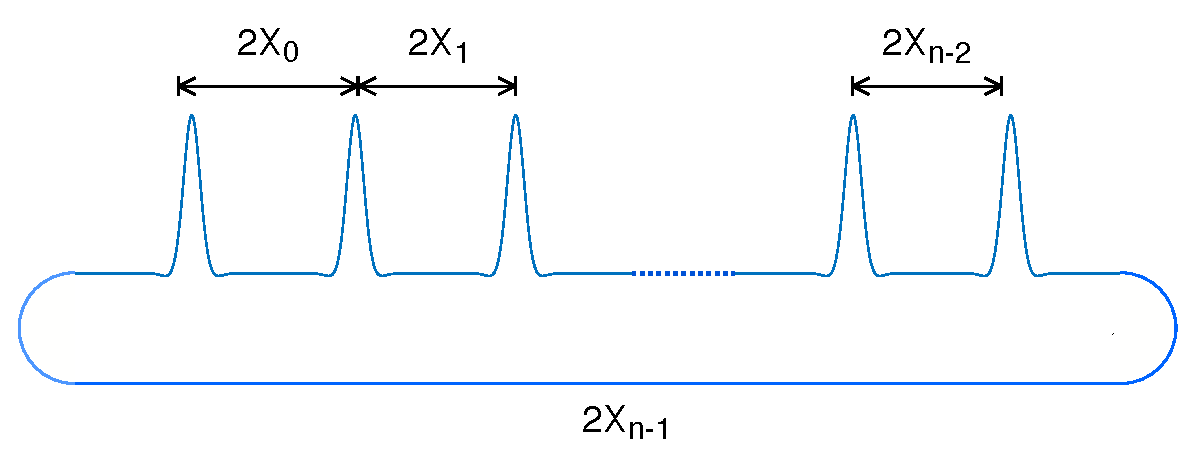
\includegraphics[width=10cm]{images/multipulseperiodic}
\end{center}
\caption[Construction of a periodic $n$-pulse solution]{Construction of a periodic $n-$pulse solution from the primary pulse.}
\label{fig:permultipulse}
\end{figure}
A periodic $n$-pulse can be described by $n$ pulse distances $\{X_0, \dots, X_{n-1} \}$, as shown in \cref{fig:permultipulse}, where the distance between consecutive copies of the primary pulse $Q(x)$ is $2 X_j$. The period of the orbit is $2X$, where $X = X_0 + \dots + X_{n-1}$. A periodic $n$-pulse requires one more pulse distance than an $n$-homoclinic orbit, since we need one more connection to ``close the loop''.  

Rather than describing a periodic multi-pulse by the pulse distances $X_j$, we will adopt an alternative parameterization which is both more mathematically convenient and captures the underlying geometry necessary for a periodic $n$-pulse to exist. This parameterization is an adaptation of that in \cite{SandstedeStrut,Sandstede1998} to the periodic case. Let
\begin{equation}\label{defrho}
\rho = \frac{\beta_0}{\alpha_0},
\end{equation}
where $\alpha_0$ and $\beta_0$ are defined in \cref{hyp:hypeq}, and let
\begin{equation}\label{pstar}
p^* = \arctan \rho.
\end{equation}
Define the set
\begin{align}
\mathcal{R} &= \left\{ \exp\left(-\frac{2 k \pi}{\rho}\right) : k \in \N_0 \right\} \cup \{ 0 \},
\end{align}
which is a complete metric space. We will use $r \in \mathcal{R}$ as a scaling parameter. The parameterization is defined as follows.

\begin{definition}\label{def:perparam}
For $n \geq 2$, a \emph{periodic parameterization} of a periodic $n$-pulse is a sequence of parameters $(m_0, \dots, m_{n-1}, \theta)$, where
\begin{enumerate}[(i)]
\item $m_j$ is a nonnegative integer with
\begin{enumerate}
\item at least one of the $m_j \in \{0, 1\}$.
\item $m_{n-1} \geq m_j$ for $j = 0, \dots, n-2$.
\end{enumerate}
\item $\theta \in (\pi + -p^*, p^*]$.
\end{enumerate}
\end{definition}
The selection of $m_{n-1}$ as the largest of the $m_j$ is made only for notational convenience and to allow the parameterization to be unique. Since we are on a periodic domain, there is no loss of generality. The physical pulse distances $X_j$ are determined by these parameters and by the scaling parameter $r$. If $r = \exp\left(-\frac{2 m \pi}{\rho}\right)$, then
\begin{align*}
X_j &= \frac{1}{2 \beta_0}\big( (2 m + m_j)\pi + \theta^*(\theta; m_{n-1} - m_j)\big) + L_0 + \mathcal{O}(r) \\
X_{n-1} &= \frac{1}{2 \beta_0}\big( (2 m + m_{n-1})\pi + \theta \big) + L_0
\end{align*}
where $L_0$ is a constant. The functions $\theta^*(\theta; m): [-\pi + p^*, p^*] \rightarrow \R$ are defined for all nonnegative integers $m$, are continuous in $\theta$, and have the following properties.
\begin{enumerate}[(i)]
\item $\theta^*(0; m) = 0 \text{ for all } m$
\item $|\theta^*(\theta; m)| \leq |\theta|$
\item $|\theta^*(\theta; m)| \leq C \exp\left(-\frac{m \pi}{\rho} \right)$
\item $\theta^*(\theta; 0) = \theta $
\item $\theta^*(p^*; m) = \theta^*(-\pi+p^*; m+1)$ for $m \geq 1$
\end{enumerate}
The last property is a matching condition which ``links up'' the parameterizations corresponding to different $m_j$. These properties, together with the restriction of $\theta$ to the half-open interval $\theta \in (\pi + -p^*, p^*]$, guarantee that each periodic parameterization corresponds to a unique periodic multi-pulse. The proof that the functions $\theta^*(\theta; m)$ exist and have these properties is given in Lemma \ref{thetaparamlemma} below.

We can now state the main theorem of this section, which gives conditions for the existence of periodic multi-pulses. The requirement that the scaling parameter $r$ be sufficiently small means that the individual pulses must be well-separated.

\begin{theorem}[Existence of $n$-periodic solutions]\label{perexist}
Assume Hypotheses \ref{hyp:E}, \ref{hyp:H}, \ref{hyp:hypeq}, \ref{Qexistshyp}, and \ref{hyp:transverse}. Let $Q(x)$ be the transversely constructed, symmetric primary pulse solution to \eqref{genODE} from Hypothesis \ref{Qexistshyp}. For any periodic parameterization $(m_0, \dots, m_{n-1}, \theta)$ with $\theta \notin \{-\pi + p^*, p^* \}$, there exists $r_* = r_*(m_0, \dots, m_{n-1}, \theta) > 0$ such that for any $r \in \mathcal{R}$ with $r \leq r_*$:
\begin{enumerate}[(i)]
	\item There exists a periodic $n$-pulse solution $U(x) = U(x; m_0, \dots, m_{n-1}, \theta, r)$ to \eqref{genODE}.

	\item The distances between consecutive copies of $Q(x)$ are $2X_j$, where
	\begin{align}\label{Xj}
		X_j(r; m_j, m_{n-1},\theta) &= \frac{1}{2 \alpha_0} |\log r| + \frac{1}{2\beta_0} t_j(r; m_j,m_{n-1}, \theta) + L_0 && j = 0, \dots, n-2 \\
		X_{n-1}(r; m_{n-1}, \theta) &= \frac{1}{2 \alpha_0} |\log r| + \frac{1}{2 \beta_0}\big( m_{n-1}\pi + \theta \big) + L_0.
	\end{align}
	The $t_j(r; m_j, m_{n-1}, \theta): \mathcal{R} \rightarrow \R$ are continuous in $r$ with 
	\[
	t_j(0; m_j, \theta) = m_j \pi + \theta^*(\theta; m_{n-1} - m_j),
	\]
	and $L_0$ is a constant.

	\item The periodic domain has length $2X$, where
	\begin{align}\label{Xdomain}
	X(r; m_0, \dots, m_{n-1}, \theta) = \frac{n}{2\alpha_0} |\log r| + \frac{1}{2\beta_0} \sum_{j=0}^{n-1} t_j(r; m_j, \theta) + n L_0
	\end{align}

	\item The specific piecewise form of $U(x)$ and estimates for $U(x)$ in terms of the primary pulse $Q(x)$ are given below in Lemma \ref{solvewithjumps}.
\end{enumerate}
\end{theorem}

\begin{remark}
It follows from the proof of \cref{2pulsebifurcation} that periodic single pulse solutions exist on domain $[-X, X]$ for all sufficiently large $X$. These are single-loop periodic orbits which lie close to the primary homoclinic orbit.
\end{remark}

The condition that $\theta \notin \{-\pi + p^*, p^*) \}$ in \cref{perexist} is used to avoid bifurcation points which arise in the construction. For periodic 2-pulses, we can use the symmetry of the solutions to give a complete bifurcation picture. In the next theorem, we show that for periodic 2-pulses, asymmetric solutions ($X_0 \neq X_1$) bifurcate from symmetric solutions ($X_0 = X_1$) in a series of pitchfork bifurcations (\cref{fig:2pitch}, left panel). \cref{2pulsebifurcation} uses a different parameterization than \cref{perexist} (\cref{fig:2pitch}, right panel).

\begin{figure}[H]
\begin{center}
\begin{tabular}{cc}
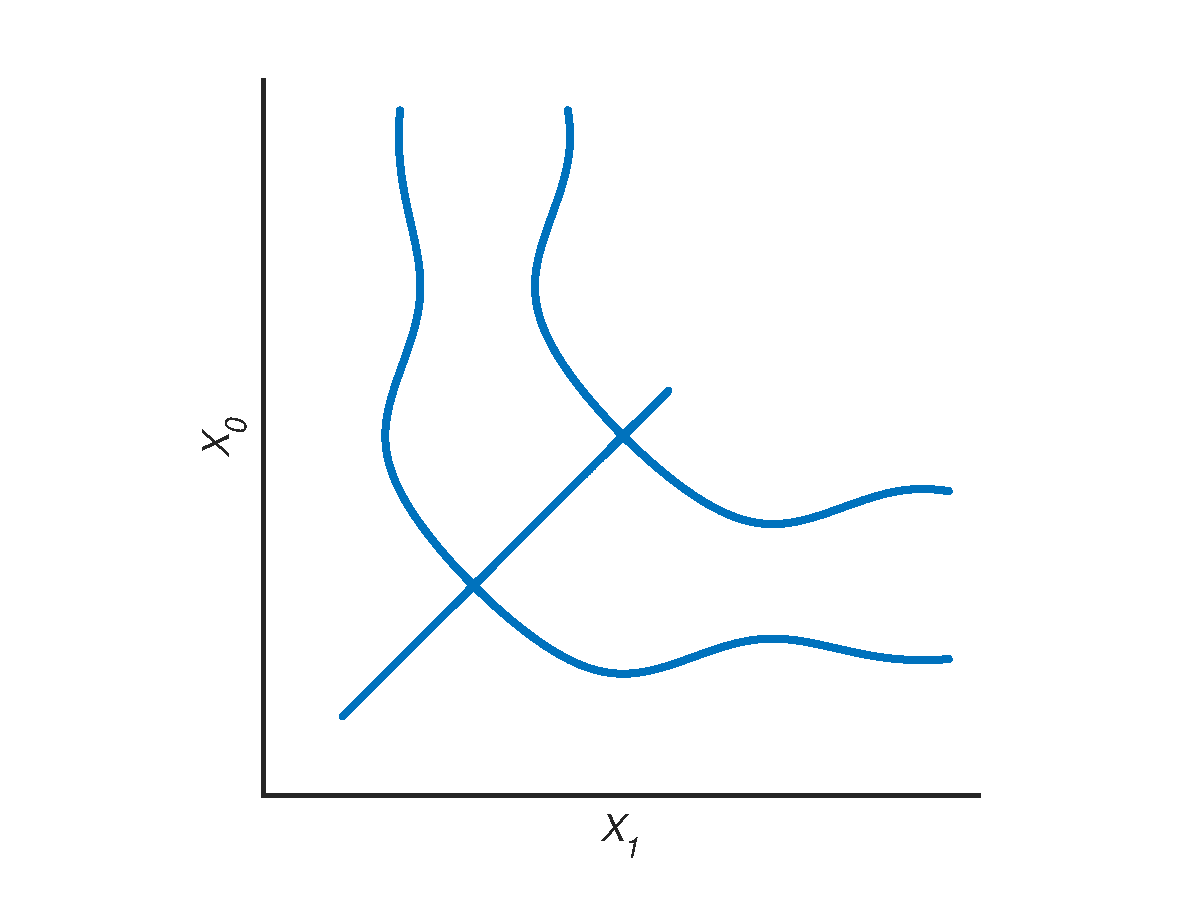
\includegraphics[width=8cm]{images/2pitchfork.eps}
\includegraphics[width=8cm]{images/2pitchparam1}
\end{tabular}
\end{center}
\caption[Pitchfork bifurcation structure for periodic 2-pulses]{Pitchfork bifurcation structure for periodic 2-pulses (right panel). Parameterization from \cref{2pulsebifurcation} (left panel). Symmetric periodic 2-pulses are in blue, and asymmetric periodic 2-pulses are in orange. Parameters $s_0$ and $s_1$ increase in the direction of the arrow.}
\label{fig:2pitch}
\end{figure} 

\begin{theorem}\label{2pulsebifurcation}
Assume Hypotheses \ref{hyp:E}, \ref{hyp:H}, \ref{hyp:hypeq}, \ref{Qexistshyp}, and \ref{hyp:transverse}. Let $Q(x)$ be the transversely constructed, symmetric primary pulse solution to \eqref{genODE} from Hypothesis \ref{Qexistshyp}. There exists $r_* > 0$ such that for all $r \in \mathcal{R}$ with $r \leq r_*$ and $m_0 \in \{0, 1\}$
\begin{enumerate}[(i)]
	\item There exists a family of symmetric periodic 2-pulses $\tilde{Q}_2(x; m_0, s_0, r)$ parameterized by $s_0 \in [0, \pi)$. The distances $\tilde{X}_j$ are given by
	\begin{equation}\label{2psymmdist}
		\tilde{X}_0(r, s_0) = \tilde{X}_1(r, s_0) = \frac{1}{2 \alpha_0} |\log r| + \frac{1}{2\beta_0} (m_0 \pi + s_0) + L_0.
	\end{equation}
	\item There exists a family of asymmetric periodic 2-pulses $Q_2(x; m_0, s_1, r)$ with distances $X_1 > X_0$ parameterized by $s_1 \in [p^*, \infty)$. The distances $X_j$ are given by
	\begin{equation}\label{2pasymmdist}
	\begin{aligned}
		X_0(r, m_0, s_1) &= \frac{1}{2 \alpha_0} |\log r| + \frac{1}{2\beta_0} t_0(r; m_0, s_1) + L_0 \\
		X_1(r, s_1) &= \frac{1}{2 \alpha_0} |\log r| + \frac{1}{2\beta_0} s_1 + L_0, 
	\end{aligned}
	\end{equation}
	where $t_0(r; m_0, s_1)$ is continuous in $r$ and $t_1$, $t_0(0; m_0, k \pi) = m_0 \pi$ for all nonnegative integers $k$, and 
	\begin{align}\label{deft0}
	t_0(0; m_0, s_1) = m_0 \pi + \mathcal{O}\left(e^{-\frac{1}{\rho} s_1 }\right).
	\end{align}

	\item The two families meet at a pitchfork bifurcation when $s_0 = p^*(m_0; r)$ and $s_1 = p^*$. The bifurcation points $p^*(m_0; r)$ are continuous in $r$, and
	\[
	p^*(m_0; r) \rightarrow \arctan \rho \text{ as }r \rightarrow 0.
	\]
\end{enumerate}
\end{theorem}

\section{Spectrum of periodic multipulses}\label{sec:perstab}

We now look at the spectrum of the periodic multi-pulses which we constructed in the previous section. Let $Q(x)$ be the primary pulse solution, and let $Q_n(x)$ be any periodic $n$-pulse solution constructed according to Theorem \ref{perexist} on periodic domain $[-X, X]$. It is natural to pose the PDE eigenvalue problem \cref{genPDEeig} on the space of periodic functions $H^{2m}_{\text{per}}[-X,X]$, where
\[
H^{2m}_{\text{per}}[-X,X] = \left\{ f \in H^{2m}(\R) : f^{(k)}(-X) = f^{(k)}(X) \text{ for } k = 0, \dots, 2m \right\} 
\]
Following the spatial dynamics approach from \cref{sec:EVP}, this is equivalent to the first order system with periodic boundary conditions
\begin{equation}\label{PDEeigsystemper3}
\begin{aligned}
V'(x) &= A(Q_n^*(x))V(x) + \lambda B V(x) \\
V(-X) &= V(X),
\end{aligned}
\end{equation}
where $V(x) \in C^0(\R,\R^{2m+1})$. Let $A(\lambda) = A(0) + \lambda B$. The next lemma states that for small $\lambda$, $A(\lambda)$ has a simple eigenvalue $\nu(\lambda)$ near 0.

\begin{lemma}\label{nulambdalemmasimple}
There exists $\delta_0 > 0$ such that for $|\lambda| < \delta_0$, the matrix $A(\lambda)$ has a simple eigenvalue $\nu(\lambda)$ near 0 given by
\begin{equation}\label{nulambda}
\nu(\lambda) = \frac{1}{c} \lambda + \mathcal{O}(|\lambda|^3)
\end{equation}
\end{lemma}

We can now state the main theorem of this section, which provides a condition for \cref{PDEeigsystemper3} to have a solution. Since the spatial dynamics formulation \cref{PDEeigsystemper3} is equivalent to the PDE eigenvalue problem, this allow us to find the eigenvalues of \cref{genPDEeig}. This theorem is analogous to \cite[Theorem 2]{Sandstede1998}, with the $n\times n$ matrix in that theorem replaced by a $2n\times 2n$ block matrix.

% block matrix theorem
\begin{theorem}\label{blockmatrixtheorem}
Assume Hypotheses \ref{hyp:E}, \ref{hyp:H}, \ref{hyp:hypeq}, \ref{Qexistshyp}, and \ref{hyp:transverse}, and \ref{hyp:dccpos}. Let $Q(x)$ be the transversely constructed, symmetric primary pulse solution to \eqref{genODE} from Hypothesis \ref{Qexistshyp}. Let $\Psi(x)$ be the solution to the adjoint variational equation from Lemma \ref{varadjsolutions}. Choose any periodic parameterization $(m_0, \dots, m_{n-1}, \theta)$ with $\theta \notin \{-\pi + p^*, p^* \}$, and let $r_*$ be as in \cref{perexist}. 

Choose any positive integer $N$. Then for any $r \leq r_*$ there exists $\delta(r,N)$, where $0 < \delta(r,N) < N/|\log r|$, with the following property. There exists a bounded, nonzero solution $V(x)$ of \cref{PDEeigsystemper3} for $|\lambda| < \delta(r,N)$ if and only if
\begin{equation}\label{blockmatrixcond}
E(\lambda) = \det S(\lambda) = 0.
\end{equation}
$S(\lambda)$ is the $(2n \times 2n)$ block matrix
\begin{equation}\label{blockeq}
S(\lambda) = 
\begin{pmatrix}
K(\lambda) -\frac{1}{2} \tilde{M} K_1(\lambda) & - \lambda^2 \tilde{M}^c I \\
-\frac{1}{2} \lambda M^c K_1(\lambda) & A - \lambda^2 MI 
\end{pmatrix}
+ \begin{pmatrix}C_1 & D_1 \\ C_2 & D_2 \end{pmatrix}
\end{equation}
The individual terms in $S(\lambda)$ are as follows.
\begin{enumerate}[(i)]
\item $K(\lambda)$ is the periodic, bi-diagonal matrix
\begin{align*}
K(\lambda) &= 
\begin{pmatrix}
e^{-\nu(\lambda)X_1} & -e^{\nu(\lambda)X_0} \\
-e^{\nu(\lambda)X_1} & e^{-\nu(\lambda)X_0}
\end{pmatrix} && n = 2 \\
K(\lambda) &=  
\begin{pmatrix}
e^{-\nu(\lambda)X_1} & & & & & -e^{\nu(\lambda)X_0} \\
-e^{\nu(\lambda)X_1} & e^{-\nu(\lambda)X_2} \\
& -e^{\nu(\lambda)X_2} & e^{-\nu(\lambda)X_3} \\
  & & \ddots & && \\
& & & & -e^{\nu(\lambda)X_{n-1}} & e^{-\nu(\lambda)X_0}
\end{pmatrix} && n > 2.
\end{align*}
$\nu(\lambda)$ is defined in Lemma \ref{nulambdalemmasimple}. $K_1(\lambda)$ is the same matrix as $K(\lambda)$ with all terms positive.

\item $A$ is the symmetric banded matrix
\begin{equation}\label{Asymm}
\begin{aligned}
A &= \begin{pmatrix}
-a_1 - a_0 & a_1 + a_0 \\
a_1 + a_0 & - a_1 - a_0 
\end{pmatrix} && n = 2 \\
A &= \begin{pmatrix}
-a_{n-1} - a_0 & a_0 & & &  & a_{n-1}\\
a_0 & -a_0 - a_1 &  a_1 \\
& a_1 & -a_1 - a_2 &  a_2 \\
& \ddots & \ddots & \ddots \\
a_{n-1} & & & & a_{n-2} & -a_{n-2} - a_{n-1} \\
\end{pmatrix} && n > 2,
\end{aligned}
\end{equation}
where
\begin{align*}
a_i &= \langle \Psi(X_i), Q'(-X_i) \rangle
\end{align*}

\item $M$, $M^c$, $\tilde{M}$, and $\tilde{M}^c$ are  Melnikov-type integrals
\begin{align*}
M &= \int_{-\infty}^\infty q(y) \partial_c q(y) dy \\
M^c &= \int_{-\infty}^\infty q(y) v^c(y) dy \\
\tilde{M} &= \int_{-\infty}^{\infty} \left(v^c(y) - \frac{1}{c}\right) dy \\
\tilde{M}^c &= \int_{-\infty}^\infty \partial_c q(y) dy .
\end{align*}
$v^c(y)$ is the first component of $V^c(y)$, which is defined in \cref{varadjsolutions}.

\item The remainder matrices are analytic in $\lambda$ and have uniform bounds
\begin{align*}
|C_1| &\leq C |\lambda|(|\lambda| + r^{1/2}) \\
|D_1| &\leq C |\lambda|(|\lambda| + r^{1/2})^2 \\
|C_2| &\leq C (|\lambda| + r^{1/2})^2 \\
|D_2| &\leq C (|\lambda| + r^{1/2})^3 
\end{align*}
The constants $C$ depend on $N$.
\end{enumerate}
\end{theorem}

\begin{remark}
In \cref{blockmatrixtheorem}, we restricted $|\lambda|$ to $|\lambda| < N/|\log r|$, for a positive integer $N$ we choose. Without this restriction, the analysis is still possible, but the remainder terms in \cref{blockeq} are much more complicated. Since the essential spectrum eigenvalues are located at approximately $c\frac{k \pi i}{X}$ for $k \in \Z$, and \begin{align*}
\left| c\frac{k \pi i}{X} \right| \leq \frac{N}{|\log r|} && |k|\leq N,
\end{align*} 
this restriction will not hinder a search for the first $N$ essential spectrum eigenvalues.
\end{remark}

\subsection{Spectrum of periodic single pulse}\label{sec:persingle}

The simplest case is the periodic single pulse. There is a only single length parameter $X_0$, which is the same as the domain length $X$. The block matrix $S(\lambda)$ is a $2\times 2$ matrix, the form of which is given in the following lemma.

\begin{lemma}\label{lemma:1blockmatrix}
For a periodic single pulse, the block matrix $S(\lambda)$ from \cref{blockmatrixtheorem} is 
\begin{align}\label{1pblockmatrix}
S(\lambda) &= 
\begin{pmatrix}
-2 \sinh(\nu(\lambda) X) - \tilde{M}\lambda \cosh(\nu(\lambda) X) & -\tilde{M}^c \lambda^2 \\
-M^c \lambda \cosh(\nu(\lambda)X) & - M \lambda^2
\end{pmatrix} +
\begin{pmatrix}
C_1 & D_1 \\ C_2 & D_2
\end{pmatrix},
\end{align}
where
\begin{align*}
|C_1|, |C_2| &\leq C |\lambda|(|\lambda| + r^{1/2}) \\
|D_1|, |D_2| &\leq C |\lambda|^2(|\lambda| + r^{1/2}).
\end{align*}
In addition,
\begin{equation}\label{1pblockmatrixdet}
\begin{aligned}
\det S(\lambda, r) &= \lambda^2 \Big( 2 M \sinh(\nu(\lambda)X)(1 + \mathcal{O}(|\lambda|^2 + r^{1/2})) + \lambda(M \tilde{M} - M_c \tilde{M}_c)\cosh(\nu(\lambda)X) \\
&\qquad+ \mathcal{O}(|\lambda|(|\lambda|^2 + r^{1/2}) \Big),
\end{aligned}
\end{equation}
and $\det S(-\lambda) = -\det S(\lambda)$.
\end{lemma}

Using this, we can compute the nonzero essential spectrum eigenvalues for the periodic single pulse. 

\begin{theorem}\label{theorem:1pess}
Assume Hypotheses \ref{hyp:E}, \ref{hyp:H}, \ref{hyp:hypeq}, \ref{Qexistshyp}, and \ref{hyp:transverse}, and \ref{hyp:dccpos}. Choose any integer $N > 0$, and let $\delta(N,r)$ be as in Theorem \ref{blockmatrixtheorem}. Then there exists $r_1 \leq r_*$ such that for any $r \in \mathcal{R}$ with $r \leq r_1$, the following holds regarding the nonzero essential spectrum eigenvalues. Let $N_1 \leq N$ be the largest positive integer such that $N_1/|\log r| < \delta(N,r)$. Then there are $2N_1$ nonzero essential spectrum eigenvalues $\lambda = \{ \pm \lambda_m^{\text{ess}} : m = 1, \dots, N_1 \}$, where
\begin{align}\label{1pess}
\lambda_m^{\text{ess}}(r) = c \frac{m \pi i}{X + c \frac{M\tilde{M} - M_c\tilde{M_c}}{2 M}} +  \mathcal{O}\left( \frac{1}{|\log r|^3} \right)
\end{align}
is on the imaginary axis.
\end{theorem}

\subsection{Spectrum of periodic double pulse}\label{sec:perdouble}

For the periodic double pulse, the block matrix $S(\lambda)$ is a $4\times 4$ matrix, the form of which is given in the next lemma.

\begin{lemma}\label{lemmma:2pblockmatrix}
For a periodic 2-pulse, the block matrix $S(\lambda)$ from \cref{blockmatrixtheorem} is the $4 \times 4$ matrix
\begin{align}\label{dpSmatrix}
S(\lambda) = 
\begin{pmatrix}
e^{-\nu(\lambda)X_1} & -e^{\nu(\lambda)X_0} & -\tilde{M}^c \lambda^2 & 0 \\
-e^{\nu(\lambda)X_1} & e^{-\nu(\lambda)X_0} & 0 & -\tilde{M}^c \lambda^2 \\
-\frac{1}{2}\lambda M^c e^{-\nu(\lambda)X_1} & -\frac{1}{2}\lambda M^ce^{\nu(\lambda)X_0} &-a-\lambda^2 M_2 & a \\
-\frac{1}{2}\lambda M^c e^{\nu(\lambda)X_1} & -\frac{1}{2}\lambda M^c e^{-\nu(\lambda)X_0}  & a & -a-\lambda^2 M_2 \\
\end{pmatrix}
+ \begin{pmatrix} C_1 & D_1 \\ C_2 & D_2 \end{pmatrix}
\end{align}
where
\begin{equation}\label{2pa}
a = \langle \Psi(X_0), Q'(-X_0) \rangle + \langle \Psi(X_1), Q'(-X_1) \rangle,
\end{equation}
the remainder matrices are $2\times2$ matrices with bounds given in \cref{blockmatrixtheorem}, and the rest of the terms are defined in \cref{blockmatrixtheorem}. In addition,
\begin{equation}\label{2pblockmatrixdet}
\begin{aligned}
\det S(\lambda, r) &= -2 \lambda^2 (2a + \lambda^2 M)\left( M \sinh(\nu(\lambda)X) + \lambda(M \tilde{M} - M_c \tilde{M}_c)\cosh(\nu(\lambda)X) \right) \\
&\qquad+ \mathcal{O}\left(|\lambda|^2(|\lambda| + r^{1/2})^4\right),
\end{aligned}
\end{equation}
and $\det S(-\lambda) = -\det S(\lambda)$.
\end{lemma}

We will consider only the case where the interaction eigenvalues are ``out of the way'' of the essential spectrum eigenvalues. Since the interaction eigenvalues scale like $r^{1/2}$ and the essential spectrum eigenvalues scale like $1/|\log r|$, we can always choose $r$ sufficiently small so that this is the case. We will state the result separately for asymmetric and symmetric periodic 2-pulses. First, we locate the eigenvalues for asymmetric 2-pulses. As long as $r$ is chosen sufficiently small, the interaction eigenvalue pattern is determined by the parameter $m_0$, and the essential spectrum eigenvalues do not interfere.

\begin{theorem}\label{theorem:2peigsassym}
Assume Hypotheses \ref{hyp:E}, \ref{hyp:H}, \ref{hyp:hypeq}, \ref{Qexistshyp}, and \ref{hyp:transverse}, and \ref{hyp:dccpos}. Let $r_*$ be as in \cref{2pulsebifurcation}. Choose any integer $N > 0$, and let $\delta(N,r)$ be as in Theorem \ref{blockmatrixtheorem}. Then for every $m_0 \in \{0, 1\}$ and $s_1 > p^*$ there exists $r_1 = r_1(m_0, s_1, N) \leq r_*$ with the following property. For any $r \in \mathcal{R}$ with $r \leq r_1$, the following hold regarding the spectrum associated with the asymmetric periodic 2-pulse $Q_2(x; m_0, s_1, r)$.

\begin{enumerate}[(i)]
\item There is an eigenvalue at 0 with algebraic multiplicity 3. 
\item Let $N_1 \leq N$ be the largest positive integer such that $N_1/|\log r| < \delta(N,r)$. Then there are $2N_1$ nonzero essential spectrum eigenvalues $\lambda = \{ \pm \lambda_m^{\text{ess}} : m = 1, \dots, N_1 \}$, where
\[
\lambda_m^{\text{ess}}(r) = c \frac{m \pi i}{X + c \frac{M\tilde{M} - M_c\tilde{M_c}}{M}} +  \mathcal{O}\left( \frac{1}{|\log r|^3} \right)
\]
is on the imaginary axis and $X$ is given by \cref{Xdomain}.

\item There is a pair of interaction eigenvalues located at $\lambda = \pm \lambda^{\text{int}}(r)$, where
	\begin{align*}
	\lambda^{\text{int}}(r) =  \sqrt{-\frac{2a}{M}} + \mathcal{O}\left( r \right),
	\end{align*}
$|\lambda^{\text{int}}(r)| < \frac{1}{2}|\lambda_1^{\text{ess}}(r)|$, and $a$ is defined in \cref{2pa}. If $M > 0$, these are real when $m_0 = 0$ and purely imaginary when $m_0 = 1$. (This is reversed if $M < 0)$. 
\item There are no other eigenvalues inside a circle with radius slightly larger than $|\lambda_{N_1}^{\text{ess}}(r)|$.
\end{enumerate}
\end{theorem}

\begin{remark}The essential spectrum eigenvalues are not identical for the periodic single pulse and the periodic double pulse. In particular, note the additional factor of 2 in the denominator of \cref{1pess}.
\end{remark}

Next, we consider the symmetric periodic 2-pulse. As long as we are away from the pitchfork bifurcation points, i.e. as long as $a \neq 0$, the results of \cref{theorem:2peigsassym} hold in the symmetric case as well; the only difference is that the eigenvalue pattern is determined by the sign of $a$ rather than by $m_0$. Thus we only need to consider what happens at the pitchfork bifurcation point.

\begin{theorem}\label{theorem:2peigssym}
Assume Hypotheses \ref{hyp:E}, \ref{hyp:H}, \ref{hyp:hypeq}, \ref{Qexistshyp}, and \ref{hyp:transverse}, and \ref{hyp:dccpos}. Then there exists $r_1 \leq r_*$ such that for all $r \in \mathcal{R}$ with $r \leq r_1$ and for $m_0 \in \{0, 1\}$, there is eigenvalue at 0 with algebraic multiplicity 5 for the symmetric periodic 2-pulse $\tilde{Q}_2(x; m_0, p^*(r), r)$.
\end{theorem}

\section{Numerical Results}\label{sec:numerics}

% In this section, we present numerical results for the existence and spectrum of periodic multi-pulse solutions to \cref{KdV5c}. We start with the construction of the primary pulse solution. For $c = 36/169 < 1/4$, an exact solution to \cref{KdV5eq4} is known \cite[(3)]{Pelinovsky2007}:
% \begin{equation}\label{KdV5exactsol}
% q(x) = \frac{105}{338}\sech^4\left(\frac{x}{2\sqrt{13}} \right)
% \end{equation}
% By \cite{Pelinovsky2007}, multi-pulses exist when $c > 1/4$, and we will show that periodic multi-pulses also exist for $c > 1/4$. To obtain a primary pulse solution for $c > 1/4$, we use AUTO for parameter continuation in $c$ starting with the solution \cref{KdV5exactsol} at $c = 36/169$. Since we will are interested in periodic solutions, we use periodic boundary conditions on the bounded interval $[-X,X]$. (To do this in AUTO, we scale equation \cref{KdV5eq4} from $[-X, X]$ to $[0, 1]$ by taking $x \mapsto \frac{1}{2X}(x + X)$). Following the AUTO demo \texttt{kdv}, we use the Hamiltonian formulation \cref{KdV5ham2} and include a small parameter $\epsilon$ to break the Hamiltonian structure. In \cref{fig:KdV5singlepulse}, we plot the exact solution (left) together with the output of parameter continuation for $c = 10$ (right). We note the presence of oscillatory tails for $c = 10$ (these are hard to see since the tails also decay exponentially, but the first downward bump is visible).
% \begin{figure}
% \begin{center}
% \begin{tabular}{cc}
% 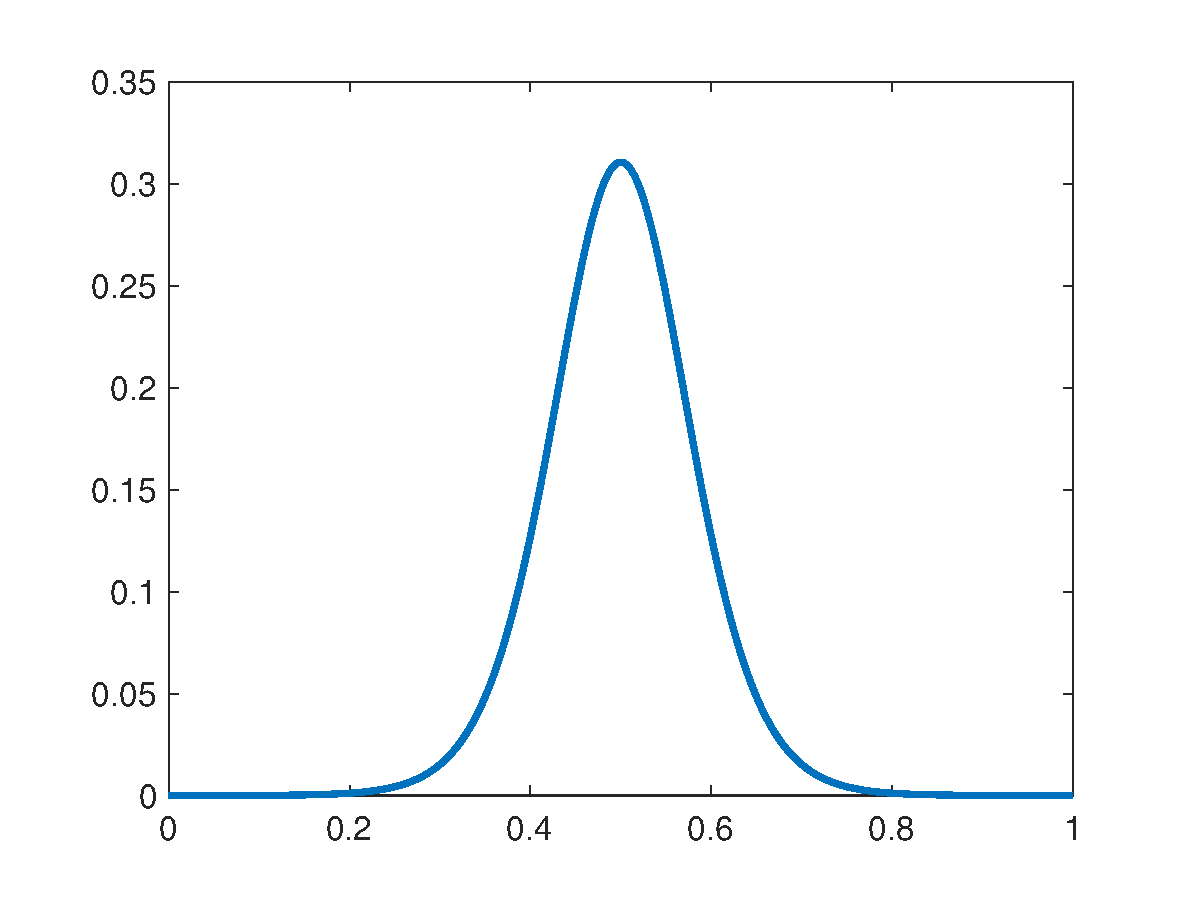
\includegraphics[width=7cm]{images/singleexact.eps} &
% 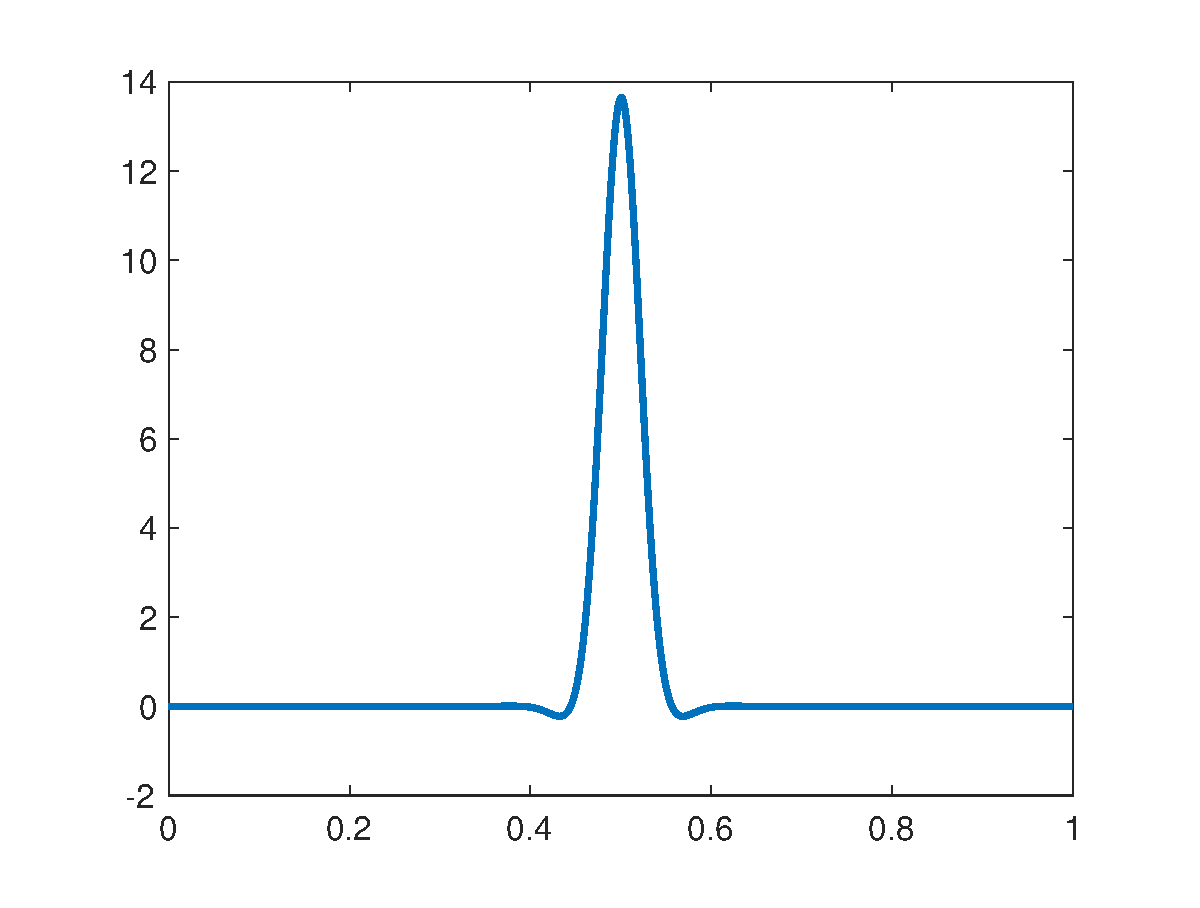
\includegraphics[width=7cm]{images/single10}
% \end{tabular}
% \caption[Primary pulse solutions for KdV5]{Single pulse solutions for KdV5. Exact solution for $c = 36/169$ (left panel) and solution from parameter continuation using AUTO for $c = 10.0$ (right panel). Solutions have been scaled to $[0, 1]$ using $X = 25$ in both cases, periodic boundary conditions.}
% \label{fig:KdV5singlepulse}
% \end{center}
% \end{figure}

% To construct a periodic double pulse, we glue together two copies of the single pulse we constructed above. To enforce periodic boundary conditions, we use Fourier spectral methods for spatial discretization. As an initial ansatz, we splice two single pulses together. For the distance between the two peaks, we use those predicted by \cite{SandstedeStrut}; we choose $X$ sufficiently large so that the tail interactions at periodic boundary conditions do not affect the solution very much. The periodic double pulse is then found using Matlab's \texttt{fsolve} function (Levenberg–Marquardt algorithm). The first six periodic double pulse solutions are shown in \cref{fig:KdV5doublepulse}.
% \begin{figure}
% \begin{center}
% 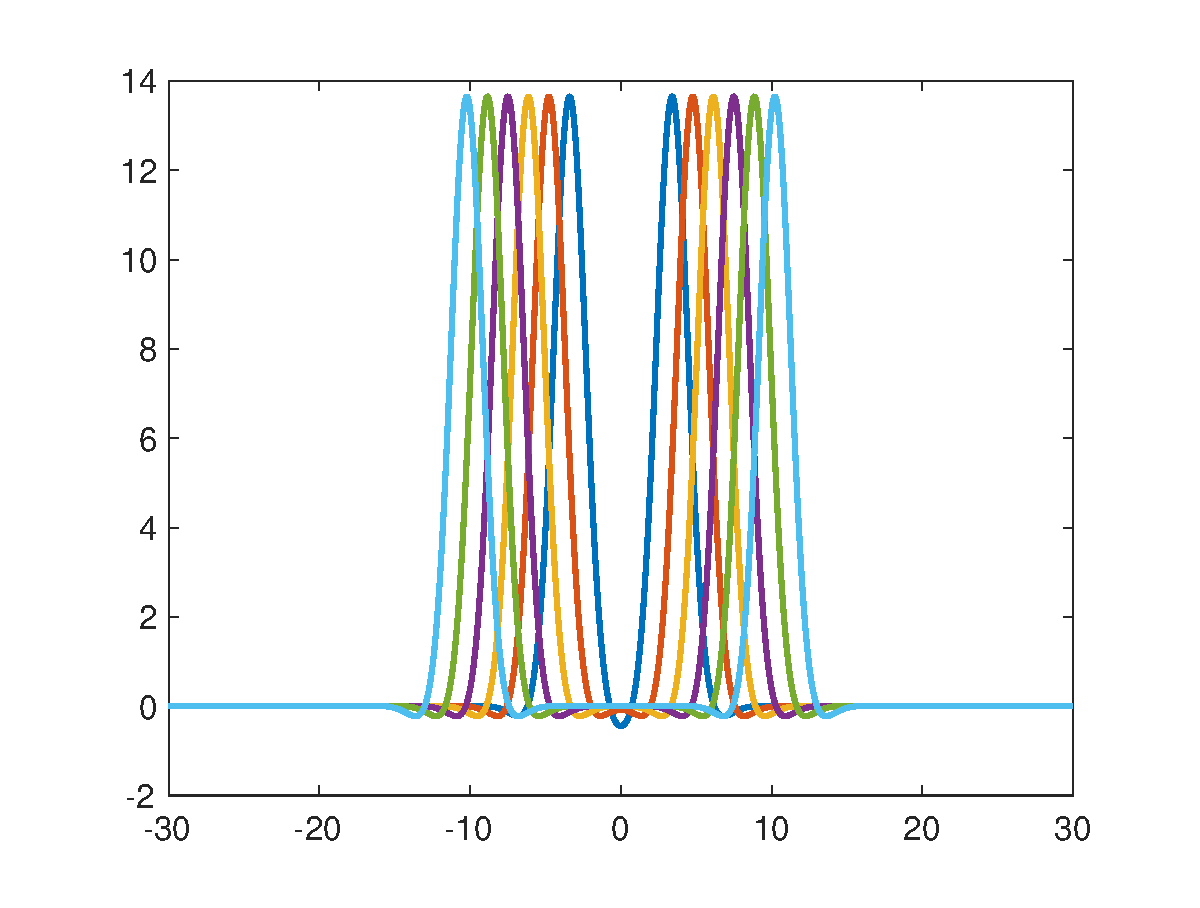
\includegraphics[width=7cm]{images/double10.eps}
% \caption[Double pulse solutions for KdV5]{First six periodic double pulse solutions for KdV5. Fourier spectral methods with $N = 1024$ grid points, $c = 10$, $X = 25$.}
% \label{fig:KdV5doublepulse}
% \end{center}
% \end{figure}
% This same procedure can be used to construct arbitrary periodic multi-pulses. Once a periodic double pulse has been constructed, we can vary $X$ by using AUTO for parameter continuation. Transforming back from the interval $[0, 1]$ to $[-X, X]$, we plot the pulse distances $2 X_0$ vs $2 X_1$ in \cref{fig:periodicpitchfork}.
% \begin{figure}
% \begin{center}
% 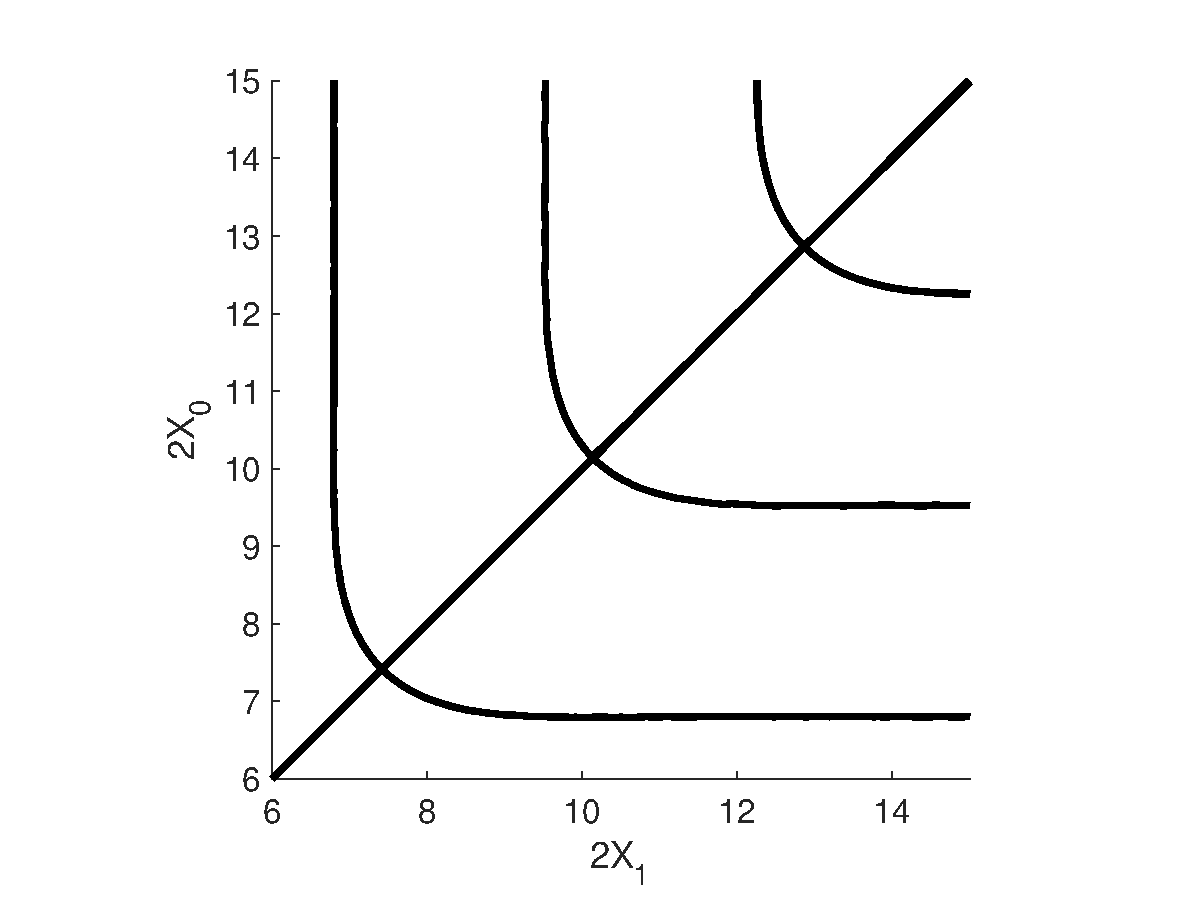
\includegraphics[width=10cm]{images/periodicpitchfork.eps}
% \end{center}
% \caption[Pulse distances of periodic multi-pulses in KdV5]{Pulse distances $2 X_0$ vs $2 X_1$ for periodic double pulse solutions to \cref{KdV5eq4}. Solutions with unequal pulse distances corresponding to the first three double pulses are shown in blue. Solutions with equal pulse distances are shown in red.}
% \label{fig:periodicpitchfork}
% \end{figure}
% From this figure, we see that solutions with unequal pulse distances bifurcate from solutions with equal pulse distances in a series of pitchfork bifurcations. 

% Now that we have constructed multi-pulses, we can look at their spectral stability. For a periodic double pulse $q_2$, we compute the spectrum of $\partial_x \calE''(q_n)$ numerically by writing the linear operator in matrix form using Fourier differentiation matrices and computing the eigenvalues of the resulting matrix using Matlab's \texttt{eig} function. On a periodic domain, the essential spectrum becomes a collection of discrete, purely imaginary eigenvalues. These eigenvalues depend only on the size of the periodic domain $X$ and are located at approximately
% \begin{equation}\label{Kdv5peress}
% \lambda \approx \left\{ c \frac{k \pi i}{L} : k \in \Z \right\} ,
% \end{equation}
% where $c$ is the wavespeed.

% Next, we compute the interaction eigenvalues for periodic double pulses with equal pulse distances. We can identify the interaction eigenvalues because they correspond to localized eigenfunctions. For periodic double pulses with equal pulse distances ($X_1 = X_2$), the result is shown in \cref{fig:periodicequaleigbif}.
% \begin{figure}
% \begin{center}
% 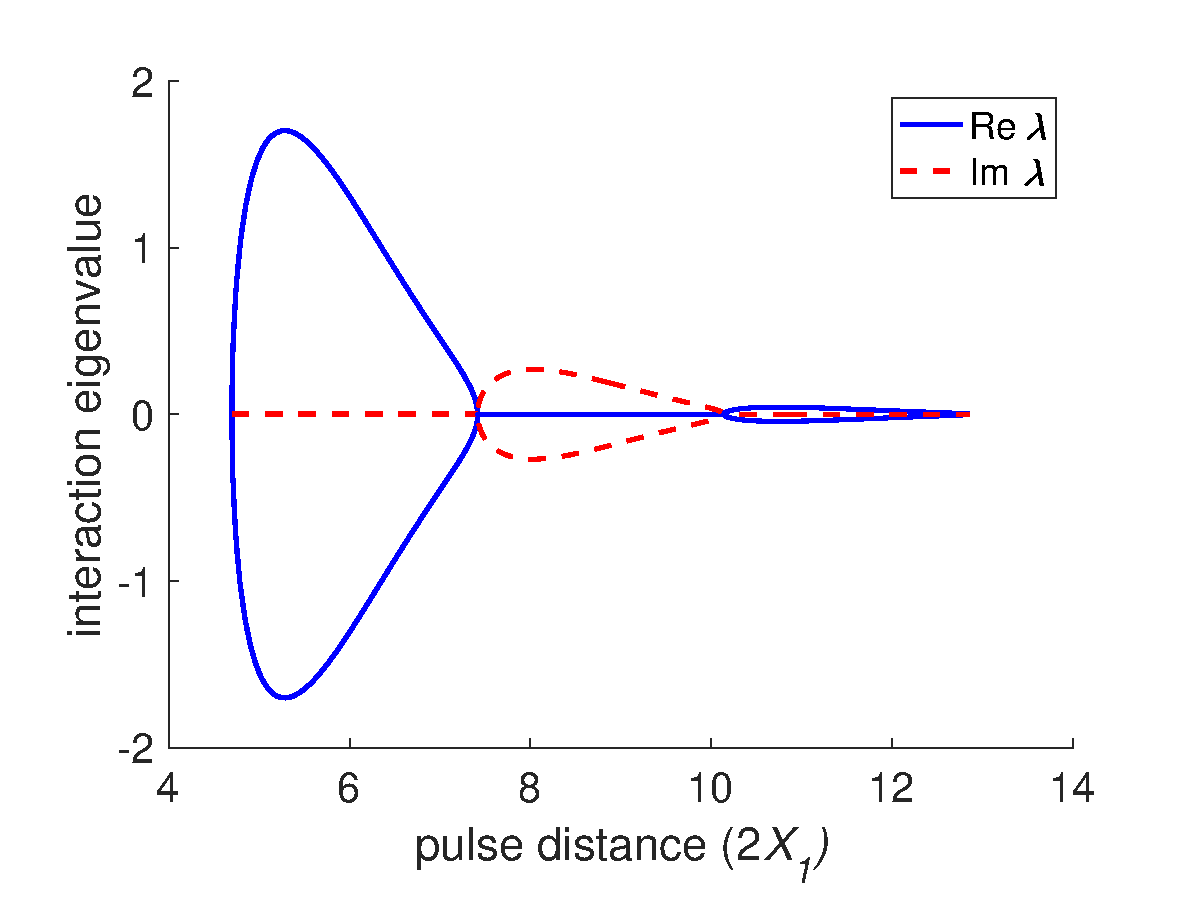
\includegraphics[width=10cm]{images/periodicequaleigbif.eps}
% \end{center}
% \caption[Eigenvalue bifurcations for symmetric periodic double pulses in KdV5]{Real (blue line) and imaginary (red line) parts of interaction eigenvalues versus pulse distance ($2 X_1$) for periodic double pulses with equal pulse distances.}
% \label{fig:periodicequaleigbif}
% \end{figure}
% At each of the pitchfork bifurcation points in \cref{fig:periodicpitchfork}, an eigenvalue bifurcation occurs, where a pair of interaction eigenvalues collides at 0 and switches from real to purely imaginary (or vice versa). The full interaction eigenvalue pattern corresponding to \cref{fig:periodicpitchfork} is given in \cref{fig:2periodiceigpattern}.
% \begin{figure}
% \begin{center}
% 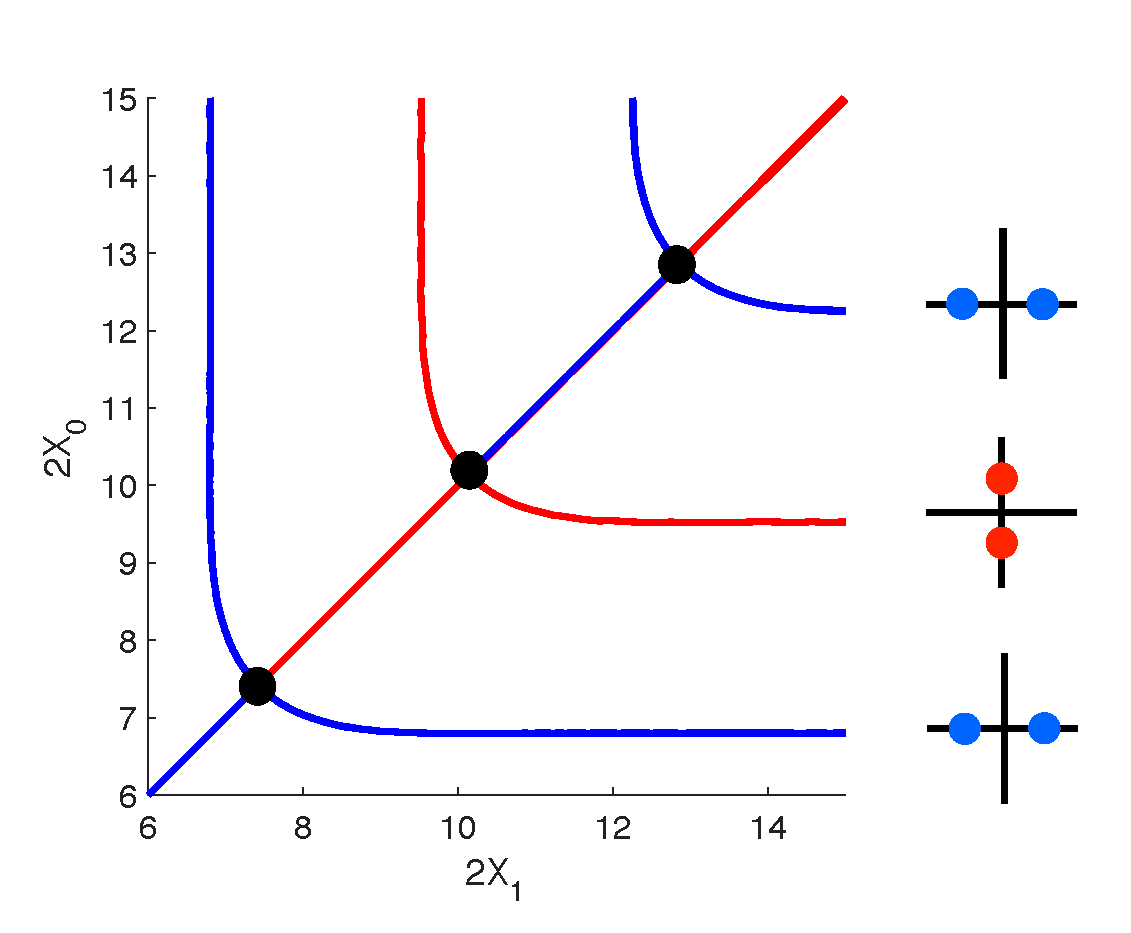
\includegraphics[width=10cm]{images/2periodiceigpattern.eps}
% \end{center}
% \caption[Interaction eigenvalue pattern for periodic double pulses in KdV5]{Interaction eigenvalue pattern for periodic double pulses. Blue lines represent periodic double pulses with a pair of real interaction eigenvalues. Red lines represent periodic double pulses with a pair of purely imaginary interaction eigenvalues. Bifurcations take place in the interaction eigenvalues at the black dots.}
% \label{fig:2periodiceigpattern}
% \end{figure}

% Finally, we look at what happens when we increase the period $X$. For a neutrally stable double pulse, we have a pair of interaction eigenvalues on the imaginary axis whose location is approximately constant for large $X$. On the other hand, the essential spectrum eigenvalues \cref{Kdv5peress} move towards the origin as $X$ is increased. It is straightforward to determine the Krein signatures of the eigenvalues numerically; the interaction eigenvalues have negative Krein signature and the essential spectrum eigenvalues have positive Krein signature. At some value of $X$, these eigenvalues will collide. When this happens, since the eigenvalues have opposite Krein signatures, the two eigenvalues will generically move off of the imaginary axis and create an instability \cite[Chapter 7.1]{Kapitula2013}. By Hamiltonian symmetry, we expect there to be a pair of eigenvalues which has nonzero real part and is symmetric across the imaginary axis.

% To see what happens in this case, we increase the periodic length parameter $X$ using AUTO. This is shown in \cref{fig:kreinbubble1}.
% \begin{figure}
% \begin{center}
% 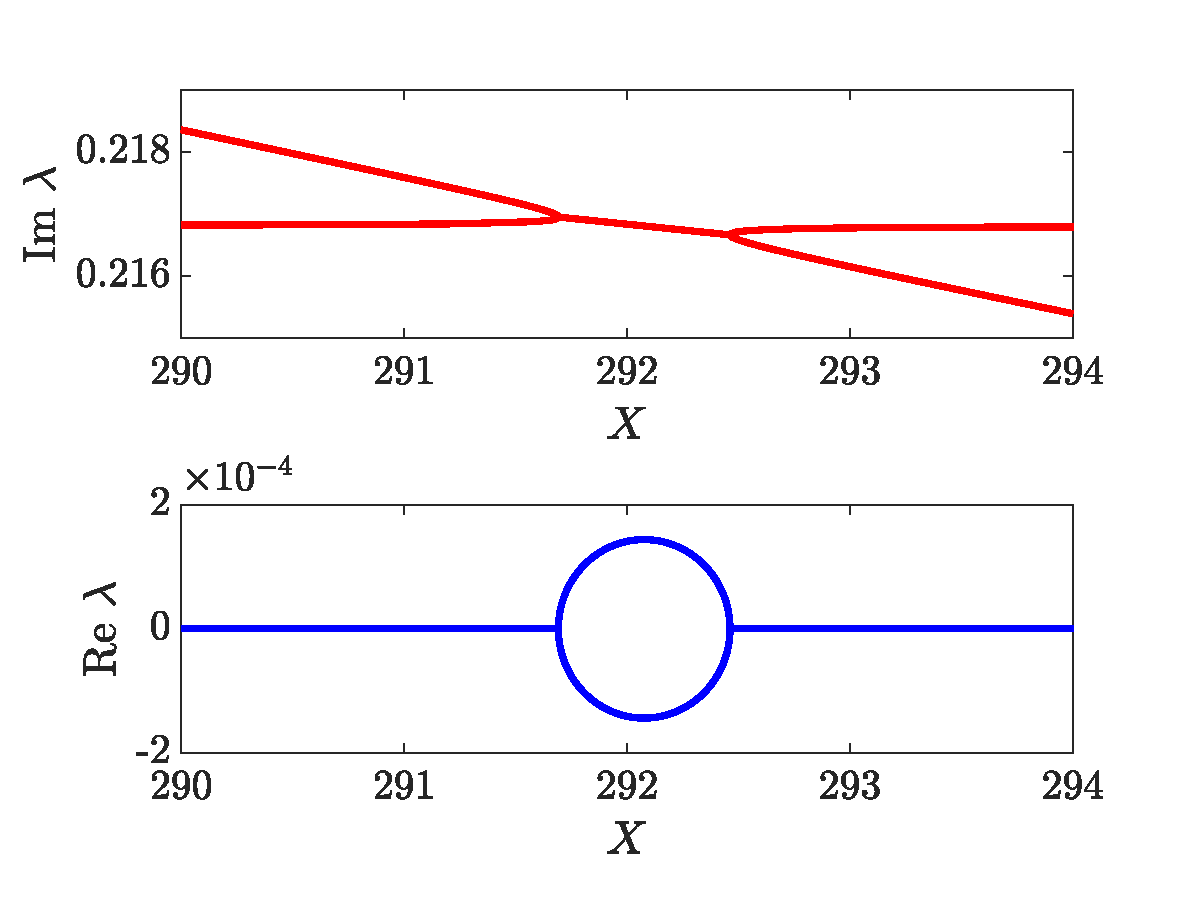
\includegraphics[width=10cm]{images/kreinbubble1}
% \end{center}
% \caption[Eigenvalue collisions for periodic double pulses in KdV5]{Collision of first essential spectrum eigenvalue with purely imaginary interaction eigenvalue as $X$ is increased. Imaginary part of eigenvalues on top, real part of eigenvalues on bottom. Parameter continuation with AUTO in periodic domain length $X$, $c = 20$.}
% \label{fig:kreinbubble1}
% \end{figure}
% As $X$ is increased, the two eigenvalues undergo a Krein collision and move off of the imaginary axis. As $X$ is further increased, the eigenvalues come back together on the imaginary axis in a reverse Krein collision. Increasing $X$ further, the essential spectrum eigenvalue continues to move on the imaginary axis towards the origin, and the interaction eigenvalue is unchanged. We will call this instability bubble a Krein bubble. \cref{fig:kreinbubble1zoom} shows the eigenvalues of the Krein bubble in the complex plane. To leading order, the bubble is a circle.
% \begin{figure}
% \begin{center}
% 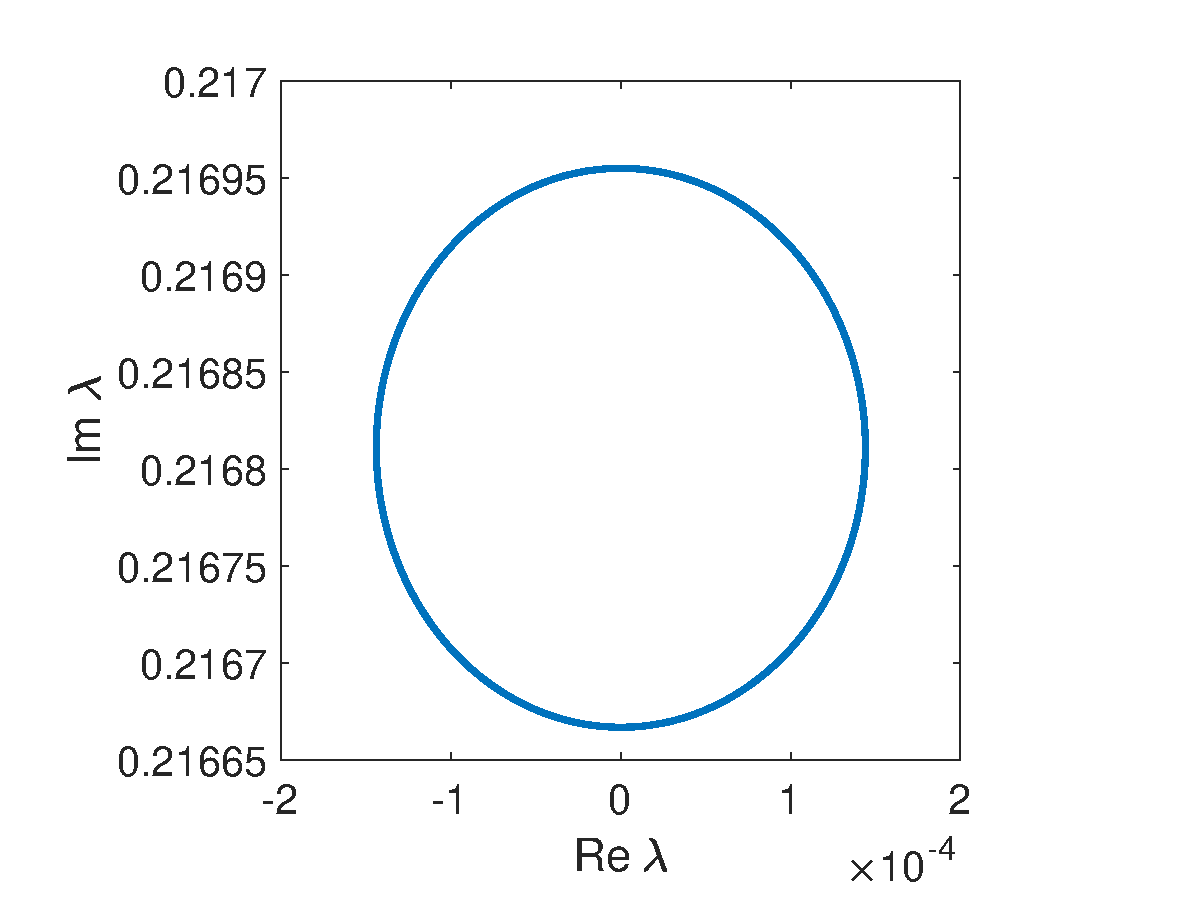
\includegraphics[width=8cm]{images/kreinbubble1zoom}
% \end{center}
% \caption[First Krein bubble for KdV5]{Plot of imaginary vs real part of eigenvalues inside Krein bubble occurring upon collision of first essential spectrum eigenvalue with interaction eigenvalue. $c = 20$.}
% \label{fig:kreinbubble1zoom}
% \end{figure}
% For $c = 20$, the maximum real part of the eigenvalues in the Krein bubble is order order $10^{-4}$, which is very small compared to the interaction eigenvalue, which is approximately $0.22i$. We can continue the parameter continuation with AUTO, and we find a Krein bubble with every subsequent collision of an essential spectrum eigenvalue with the interaction eigenvalue. \cref{fig:kreinbubbleradius} plots the log of the Krein bubble radius versus the log of $X$ for the first 10 Krein bubbles.
% \begin{figure}
% \begin{center}
% 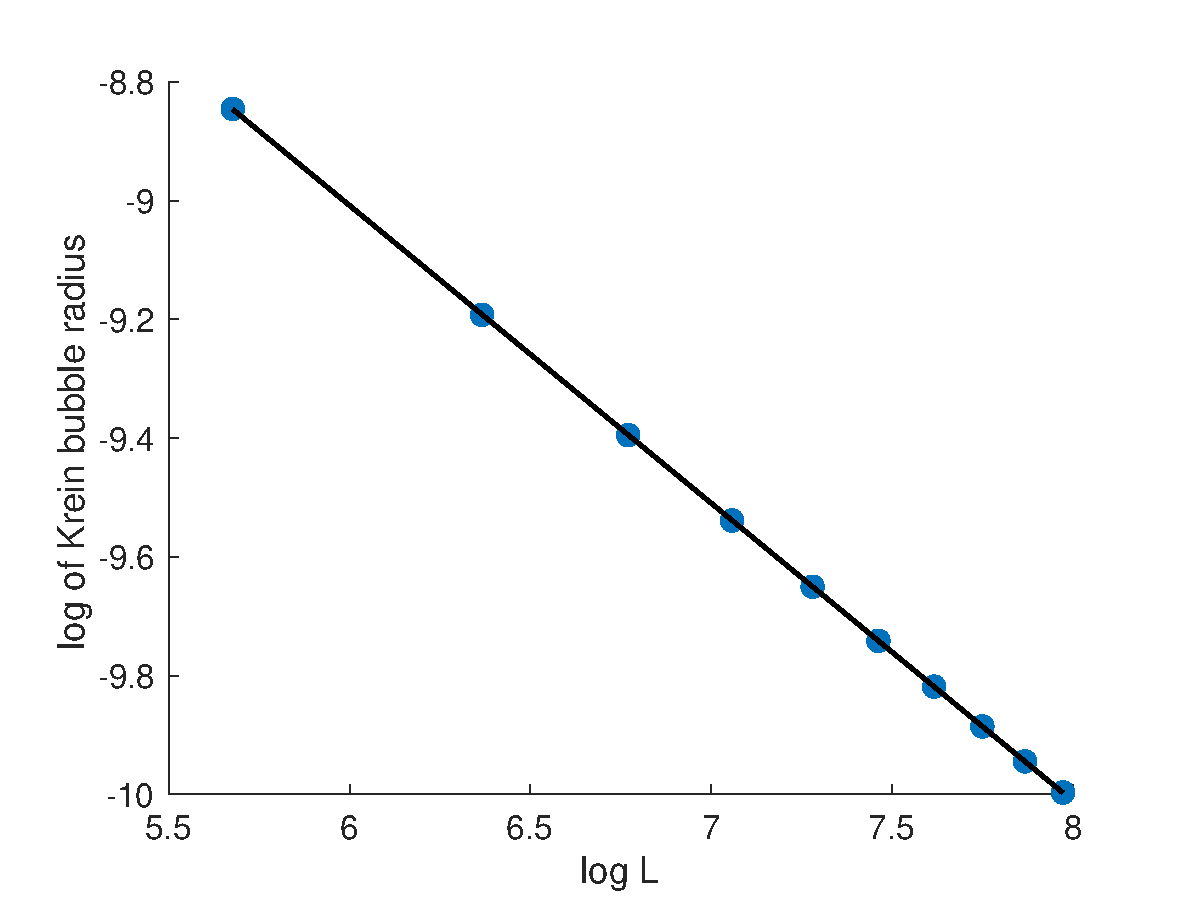
\includegraphics[width=8cm]{images/kreinbubbleradius}
% \end{center}
% \caption[Krein bubble radius for KdV5]{Plot of log of Krein bubble radius vs. log $X$ for the first 10 Krein bubbles together with least squares linear regression line. $c = 20$.}
% \label{fig:kreinbubbleradius}
% \end{figure}
% The slope of the least squares linear regression line is $-0.5$ (with a relative error of less than $0.005$), which suggests that the radius of the Krein bubble scales as $X^{-1/2}$

\section{Conclusions}\label{sec:conclusions}

\appendix

\section{Proof of existence results}\label{sec:existproof}

We will construct periodic multi-pulses using Lin's method. Rather than constructing a periodic $n$-pulse $U(x)$ as a piecewise perturbation of the primary pulse $Q(x)$, we adapt the technique in \cite{Sandstede1997} and take a piecewise ansatz of the form
\[
U_i^\pm(x) = Q^\pm(x; \beta_i^\pm) + \tilde{Q}_i^\pm(x),
\]
where the functions $Q^\pm(x; \beta_i^\pm)$ paramaterize the stable and unstable manifolds $\tilde{W}^s(0)$ and $\tilde{W}^u(0)$ near $Q(0)$, and $\tilde{Q}_i^\pm$ are small remainder terms. In essence, we use the small parameters $\beta_i^\pm$ to break the homoclinic orbit $Q(x)$, and then use Lin's method to glue the pieces together. We will show that we can find a unique piecewise solution $U_i^\pm(x)$ which generically has $n$ jumps in a specified direction. A periodic multi-pulse solution exists if and only if these $n$ jumps are all 0.

\subsection{Setup}

Using \cref{nondegencond}, we decompose the tangent spaces of the stable and unstable manifolds at $Q(0)$ as 
\begin{equation*}
\begin{aligned}
T_{Q(0)}\tilde{W}^u(0) &= \R Q'(0) \oplus Y^- \\
T_{Q(0)}\tilde{W}^s(0) &= \R Q'(0) \oplus Y^+
\end{aligned}
\end{equation*}
The variational and adjoint variational equations associated with \cref{genODE} are
\begin{align}
V' = DF(Q(x)) V \label{vareq1} \\
W' = -DF(Q(x))^* W \label{adjvareq1},
\end{align}
It follows from \cref{nondegencond} that $Q'(x)$ is the unique bounded solution to \cref{vareq1}, and that there exists a unique bounded solution $\Psi(x)$ to \cref{adjvareq1}. (In both cases, uniqueness is up to scalar multiples). Since we have a conserved quantity $H$, the following lemma gives the exact form of $\Psi(x)$.

\begin{lemma}\label{psiform}
We can take $\Psi(x) = \nabla H(Q(x))$, where $H$ is the conserved quantity from \cref{hyp:H}. In addition, $\Psi(-x) = R \Psi(x)$, where $R$ is the standard reversor operator, and the last component of $\Psi(x)$ is $q'(x)$.
\begin{proof}
Taking the gradient of \cref{HFperp}, we have $0 = D F(Q(x))^* \nabla H(Q(x)) + D^2 H(Q(x))^* F(Q(x))$. Using standard vector calculus identities, equation \cref{eqODE}, and the fact that the Hessian is self-adjoint,
\begin{align*}
-D F(Q(x))^* \nabla H(Q(x)) &= D^2 H(Q(x)) Q'(x) = \frac{d}{dx} \nabla H(Q(x))
\end{align*}
thus $\nabla H(Q(x))$ is a solution to \eqref{adjvareq1}. Since $\nabla H$ is continuous and $Q(x)$ is exponentially localized, $\nabla H(Q(x))$ is bounded as well, thus by uniqueness we can take $\Psi(x) = \nabla H(Q(x))$. Using \eqref{genODErev} and the symmetry relation $Q(-x) = R Q(x)$, 
\begin{align*}
[R \Psi(-x)]' = -R DF(Q(-x)) \Psi(-x) 
= -R [-RDF(Q(x))R] \Psi(-x) = DF(Q(x))[ R \Psi(-x) ].
\end{align*}
By uniqueness, $\Psi(x) = R \Psi(-x)$, thus $\Psi(-x) = R \Psi(x)$. By the construction of $F$, if $\Psi(x) = (\psi_1(x), \dots, \psi_{2m}(x))$ is a solution to \cref{adjvareq1}, then $\psi_{2m}(x)$ solves $\calL(q)^* w = [\calE''(q) + c]^* w = 0$. Since $\calL(q)$ is self-adjoint and $\calL(q)q' = 0$, by uniqueness we must have $\psi_{2m}(x) = q'(x)$.
\end{proof}
\end{lemma}

In the next lemma, we collect a few important results about solutions to \cref{vareq1} and \cref{adjvareq1}.

\begin{lemma}\label{eigadjoint}
Consider the linear ODE $V' = A(x)V$ and the corresponding adjoint equation $W' = -A(x)^* W$, where $A(x)$ is a smooth $n \times n$ matrix. Then
\begin{enumerate}[(i)]
\item $\dfrac{d}{dx}\langle V(x), W(x) \rangle = 0$, thus the inner product is constant in $x$.
\item If $W(x)$ is bounded and $V(x) \rightarrow 0$ as $x \rightarrow \infty$ or $x \rightarrow -\infty$, then $\langle V(x), W(x) \rangle = 0$ for all $x \in \R$. The same holds if we reverse the roles of $W$ and $V$.
\item If $\Phi(y, x)$ is the evolution operator for $V'(x) = A(x)V(x)$, then $\Phi(x, y)^*$ is the evolution operator for the adjoint equation $W'(y) = -A(y)^* W(y)$.
\end{enumerate}
\begin{proof}
For part (i), 
\begin{align*}
\dfrac{d}{dx}\langle V(x), W(x) \rangle &= 
\langle V'(x), W(x) \rangle + \langle V(x), W'(x) \rangle \\
&= \langle A(x)V(x), W(x) \rangle + \langle V(x), -A(x)^* W(x) \rangle = 0
\end{align*}
Part (ii) follows from part (i), the Cauchy-Schwartz inequality and the continuity of the norm. For part (iii), take the derivative of the expression $\Phi(y, x)\Phi(x, y) = I$ with respect to $y$ to get
\begin{align*}
0 &= \left(\frac{d}{dy}\Phi(y, x)\right) \Phi(x, y) +
\Phi(y, x)\left(\frac{d}{dy}\Phi(x, y)\right) 
= A(y) + \Phi(y, x)\left(\frac{d}{dy}\Phi(x, y)\right).
\end{align*}
Rearrange and take the transpose of both sides to get
\begin{align*}
\frac{d}{dy}\Phi(x, y)^* &= -A(y)^* \Phi(x, y)^*  
\end{align*}
\end{proof}
\end{lemma}

\noi Using \cref{eigadjoint}(ii), $\Psi(0) \perp \R Q'(0) \oplus Y^+ \oplus Y^-$, thus we can decompose $\R^{2m}$ as
\begin{equation}\label{R2mdecomp}
\R^{2m} = \R Q'(0) \oplus Y^+ \oplus Y^- \oplus \R \Psi(0).
\end{equation}

\subsection{Piecewise ansatz}

First, we write the manifolds $\tilde{W}^u(0)$ and $\tilde{W}^s(0)$ as graphs over their tangent spaces near $Q(0)$. Following \cite{Sandstede1997}, we can parameterize the unstable and stable manifolds near $Q(0)$ by the smooth functions $Q^-(\gamma, \beta^-)$ and $Q^+(\gamma, \beta^+)$, where $\gamma \in \R$, $\beta^\pm \in Y^\pm$. These functions are chosen so that $Q^+(\gamma, 0) - Q^-(\gamma, 0) \in \R \Psi(0)$, and $Q^+(0, 0) = Q^-(0, 0) = Q(0)$. We will always take $\gamma = 0$. Let $Q^\pm(x; \beta^\pm)$ be the unique solutions to \eqref{genODE} on $\R^\pm$ with initial conditions $Q^\pm(0, \beta^\pm)$ at $x = 0$. We will look for a $n-$periodic solution $U(n)$ to \eqref{genODE} which is piecewise of the form
\begin{equation}\label{Upiecewise}
\begin{aligned}
U_i^-(x) &= Q^-(x; \beta_i^-) + \tilde{Q}_i^-(x) && x \in [-X_{i-1}, 0] \\
U_i^+(x) &= Q^+(x; \beta_i^+) + \tilde{Q}_i^+(x) && x \in [0, X_i]
\end{aligned}
\end{equation}
for $i = 0, \dots, n-1$, where $U_i^-: [-X_{i-1}, 0] \rightarrow \R$ and $U_i^+: [0, X_i] \rightarrow \R$ are continuous. The subscripts $i$ are taken $\Mod n$ since we are on a periodic domain, and the pieces are glued together end-to-end as in \cite{Sandstede1998} 
. Since $Q^\pm(0; \beta_i^\pm) \in \R Q'(0) \oplus Y^\pm$, we are free to choose $\tilde{Q}_i^\pm(x)$ such that
\begin{align*}
\tilde{Q}_i^-(0) &\in \R \Psi(0) \oplus Y^- \\
\tilde{Q}_i^+(0) &\in \R \Psi(0) \oplus Y^+
\end{align*}
In order to construct a periodic $n$-pulse, i.e. to join the $2n$ pieces $U_i^\pm(x)$ end-to-end in a loop, we will solve the following system of equations
\begin{align}
(U_i^\pm(x))' - F(U_i^\pm(x)) &= 0 \label{exsystem1} \\
U_i^+(X_i) - U_{i+1}^-(-X_i) &= 0 \label{exsystem2} \\
U_i^+(0) - U_i^-(0) &= 0 \label{exsystem3}
\end{align}
for $i = 0, \dots, n-1$. Equation \cref{exsystem2} is a matching condition at the pulse tails, and equation \cref{exsystem3} is a matching condition at the pulse centers.

\subsection{Exponential Dichotomy}\label{sec:existdichot}

Let $\Phi_\pm(x, y; \beta^\pm)$ be the family of evolution operators for
\begin{align}\label{qpmODEs}
[V^\pm(x)]' &= D F\left(Q^\pm(x, \beta^\pm)\right) V^\pm(x) && x \in \R^\pm
\end{align}
Choose any $\alpha$ slightly less than $\alpha_0$. In the next lemma, we decompose these evolution operators in exponential dichotomies on $\R^+$ and $\R^-$. 

% lemma : exp dichotomy
\begin{lemma}\label{dichotomy1}
There exist projections
\begin{align*}
&P_+^s(y; \beta^+) && y \geq 0 \\
&P_+^u(y; \beta^+) = I - P_+^s(y; \beta^+) && y \geq 0 \\
&P_-^u(y; \beta^-) && y \leq 0 \\
&P_-^s(y; \beta^-) = I - P_-^u(y; \beta^-) && y \leq 0 \\
\end{align*}
such that the evolution operators $\Phi_\pm(x, y; \beta^\pm)$ can be decomposed as
\begin{align*}
\Phi^s_\pm(x, y; \beta^\pm) &= \Phi_\pm(x, y; \beta^\pm) P^s_\pm(y; \beta^\pm) \\
\Phi^u_\pm(x, y; \beta^\pm) &= \Phi_\pm(x, y; \beta^\pm) P^u_\pm(y; \beta^\pm),
\end{align*}
and we have the estimates
\begin{align*}
|\Phi^s_+(x, y, \beta^+)| &\leq C e^{-\alpha(x - y)} && 0 \leq y \leq x \\
|\Phi^u_+(x, y, \beta^+)| &\leq C e^{-\alpha(y - x)} && 0 \leq x \leq y \\
|\Phi^u_-(x, y, \beta^-)| &\leq C e^{-\alpha(y - x)} && 0 \geq y \geq x \\
|\Phi^s_-(x, y, \beta^-)| &\leq C e^{-\alpha(x - y)} && 0 \geq x \geq y \\
\end{align*}
which also hold for derivatives with respect to the initial conditions $\beta^\pm$. In addition, the projections satisfy the commuting relations
\begin{align*}
\Phi_\pm(x, y; \beta^\pm) P^{s/u}_\pm(y; \beta^\pm) 
= P^{s/u}_\pm(x; \beta^\pm) \Phi_\pm(x, y; \beta^\pm)
\end{align*}
The projections can be chosen such that at $y = 0$ we have, independent of $\beta^+$ and $\beta^-$
\begin{align*}
\ker P^s_+(0; \beta^+) &= \R \Psi(0) \oplus Y^- \\
\ker P^u_-(0; \beta^-) &= \R \Psi(0) \oplus Y^+ \\
\ran P^u_+(0; \beta^+) &= \R \Psi(0) \oplus Y^- \\
\ran P^s_-(0; \beta^-) &= \R \Psi(0) \oplus Y^+
\end{align*}
Let $E_0^s$ and $E_0^u$ be the stable and unstable eigenspaces of $DF(0)$, and let $P_0^s$ and $P_0^u$ be the corresponding eigenprojections. Then
\begin{equation}\label{projdiffest}
\begin{aligned}
|P^u_+(x; \beta^+) - P_0^u| &\leq C e^{-\alpha x} \\
|P^s_+(x; \beta^+) - P_0^s| &\leq C e^{-\alpha x} \\
|P^u_-(x; \beta^-) - P_0^u| &\leq C e^{\alpha x} \\
|P^s_-(x; \beta^-) - P_0^s| &\leq C e^{\alpha x} 
\end{aligned}
\end{equation}
These estimates are independent of $\beta_i^\pm$.

\begin{proof}
Since $DF(0)$ is hyperbolic by \cref{hyp:hypeq} and $|\Re \nu| \geq \alpha_0$ for all eigenvalues $\nu$ of $DF(0)$, the exponential dichotomy results follow from \cite[Lemma 5.1]{Sandstede1997}, which follows from \cite[Lemma 1.1]{Sandstede1993}. The estimates \cref{projdiffest} follow from \cite[Lemma 1.1]{Sandstede1993} and \cite[Lemma 2.1]{Sandstede1993}.
\end{proof}
\end{lemma}

\subsection{Fixed Point Formulation}

Next, we formulate equation \eqref{exsystem1} as a fixed point problem. Plug in the piecewise ansatz \eqref{Upiecewise} into \eqref{genODE} and using the fact that $Q^\pm(x; \beta_i^\pm)$ solves \eqref{genODE} on $\R^\pm$,
\begin{align*}
(\tilde{Q}_i^\pm(x))' &= F\left(Q^\pm(x; \beta_i^\pm) + \tilde{Q}_i^\pm(x) \right) - F(Q^\pm(x; \beta_i^\pm)) && i = 0, \dots, n-1
\end{align*}
Expanding the RHS in a Taylor series about $Q^\pm(x; \beta_i^\pm)$, we obtain the ODE for $\tilde{Q}_i^\pm$
\begin{align}\label{Vpiecewise1}
(\tilde{Q}_i^\pm(x))' &= DF(Q^\pm(x; \beta_i^\pm)) \tilde{Q}_i^\pm(x) + G_i^\pm(x; \beta_i^\pm) && i = 0, \dots, n-1
\end{align}
where
\begin{equation}\label{Gquadratic}
G_i^\pm(x; \beta_i^\pm) = \mathcal{O}(|\tilde{Q}_i^\pm(x)|^2).
\end{equation}
As in \cite{Sandstede1997}, derivatives of $G_i^\pm$ with respect to the parameters $\beta_i^\pm$ are also quadratic in $\tilde{Q}_i^\pm$. We rewrite \eqref{Vpiecewise1} in integrated form to get the fixed point problem
\begin{equation}\label{FPequations}
\begin{aligned}
\tilde{Q}_i^+(x) &= \Phi^u_+(x, X_i; \beta_i^+) a_i^+  
+ \int_{X_i}^x \Phi_+^u(x, y; \beta_i^+) G_i^+(y; \beta_i^+)dy 
+ \int_0^x \Phi_+^s(x, y; \beta_i^+) G_i^+(y; \beta_i^+)dy \\ 
\tilde{Q}_i^-(x) &= \Phi^s_-(x, -X_{i-1}; \beta_i^-) a_{i-1}^-  
+\int_{-X_{i-1}}^x \Phi_-^s(x, y; \beta_i^-) G_i^-(y; \beta_i^-)dy 
+ \int_0^x \Phi_-^u(x, y; \beta_i^-) G_i^-(y; \beta_i^-)dy
\end{aligned}
\end{equation}
where $a_i^+ \in E_0^u$ and $a_i^- \in E_0^s$. Define the exponentially weighted norms
\begin{equation}\label{expwtnorm}
\begin{aligned}
\|V\|_{X, +} &= \sup_{x \in [0, X]} e^{\alpha(X - x)}|V(x)| \\
\|V\|_{X, -} &= \sup_{x \in [-X, 0]} e^{\alpha(X + x)}|V(x)|,
\end{aligned}
\end{equation}
and let $K_{X, \pm}$ be the Banach spaces of continuous functions on $[0, X]$ and $[-X, 0]$ equipped with these norms. Let $B_{X, \pm}(\rho)$ be the ball of radius $\rho$ about $0$ in $K_{X, \pm}$.

\subsection{Inversion}

As in \cite{Sandstede1997}, we will solve for the remainder functions $\tilde{Q}_i^\pm$ and parameters $\beta_i^\pm$ in a series of lemmas. First, we will solve equation \cref{exsystem1} for $\tilde{Q}_i^\pm(x)$.

\begin{lemma}\label{solveforV}
There exist $\delta, \rho > 0$ such that for $|X_i|, |X_{i-1}| > 1/\delta$ and $|a_{i-1}^-|, |a_i^+|, |\beta_i^\pm| < \delta$, there exist unique solutions
\begin{align*}
\tilde{Q}_i^-(a_{i-1}^-, \beta_i^-) &\in B_{X_{i-1}, -}(\rho) \\
\tilde{Q}_i^+(a_i^+, \beta_i^+) &\in B_{X_i, +}(\rho) \\
\end{align*}
to \eqref{FPequations}. $\tilde{Q}_i^-(a_{i-1}, \beta_i^-)$ depends smoothly on $(a_{i-1}^-, \beta_i^-)$, and $\tilde{Q}_i^+(a_i, \beta_i^+)$ depends smoothly on $(a_i^+, \beta_i^+)$, and we have the estimates
\begin{equation}\label{Vest}
\begin{aligned}
\|\tilde{Q}_i^-\|_{X_{i-1}, -} &\leq C |a_{i-1}^-| \\
\|\tilde{Q}_i^+\|_{X_i, +} &\leq C |a_i^+|
\end{aligned}
\end{equation}
where the constant $C$ depends only on $\delta$. The estimates hold for derivatives of $\tilde{Q}_i^\pm$ with respect to $\beta_i^\pm$.
\begin{proof}
The proof follows \cite[Lemma 5.2]{Sandstede1997}. For the first term on the RHS of \eqref{FPequations} on $\R^+$,
\begin{align*}
e^{\alpha(X_i - x)} | \Phi^u_+(x, X_i; \beta_i^+) a_i^+ | 
&\leq C e^{\alpha(X_i - x)} e^{-\alpha(X_i - x)} |a_i^+| = C |a_i^+|,
\end{align*}
and for the second term, since $G_i^+$ is quadratic order in $\tilde{Q}_i^+$ and $\tilde{Q}_i^+ \in K_{X_i, +}$, 
\begin{align*}
e^{\alpha(X_i - x)} &\left| \int_{X_i}^x \Phi_+^u(x, y; \beta_i^+) G_i^+(y; \beta_i^+)dy  \right| 
\leq C e^{\alpha(X_i - x)} \int_x^{X_i} e^{-\alpha(y - x)}|\tilde{Q}_i^+(y)|^2 dy \\
&\leq C e^{\alpha(X_i - x)} \int_x^{X_i} 
e^{-\alpha(y - x)}(e^{-\alpha(X_i - y)})^2|e^{\alpha(X_i - y)} \tilde{Q}_i^+(y)|^2 dy \leq C
\end{align*}
The third term is similarly bounded. Thus the RHS of the fixed point equation \eqref{FPequations} on $\R^+$ is a smooth map $K_{X_i, +} \mapsto K_{X_i, +}$. Define $H: K_{X_i, +} \times E_0^s \times Y^+ \rightarrow K_{X_i, +}$ by
\begin{align*}
H(\tilde{Q}_i^+(x), &a_i^+, \beta_i^+) = \tilde{Q}_i^+(x) - \Phi^u_+(x, X_i; \beta_i^+) a_i^+ - \int_{X_i}^x \Phi_+^u(x, y; \beta_i^+) G_i^+(y; \beta_i^+)dy \\
&- \int_0^x \Phi_+^s(x, y; \beta_i^+) G_i^+(y; \beta_i^+)dy.
\end{align*}
Since $Q(x)$ satisfies \eqref{genODE}, $H(0, 0, 0) = 0$, and since $G_i^+$ is quadratic in $\tilde{Q}_i^+(x)$, the Fr\'echet derivative of $H$ with respect to $\tilde{Q}_i^+(x)$ at $(\tilde{Q}_i^+(x), a_i^+, \beta_i^+) = (0, 0, 0)$ is the identity. Using the implicit function theorem, we can solve for $\tilde{Q}_i^+(x)$ in terms of $(a_i^+, \beta_i^+)$ for sufficiently small $|a_i^+|$ and $|\beta_i^+|$. Since the map $H$ is smooth, this dependence is smooth. The estimate on $\tilde{Q}_i^+$ comes from the first term on the RHS of \eqref{FPequations}, since the remaining terms on the RHS are are quadratic in $\tilde{Q}_i^+$. Since the exponential dichotomy estimates from Lemma \ref{dichotomy1} hold for derivatives with respect to $\beta_i^+$, these do as well. We can similary solve for $\tilde{Q}_i^-$ in terms of $(a_{i-1}^-, \beta_i^-)$.
\end{proof}
\end{lemma}

Next, we will solve equation \cref{exsystem2} to match the pieces \cref{Upiecewise} at $\pm X_i$, which will solve for the initial conditions $a_i^\pm$.

\begin{lemma}\label{solvefora}
For $X_i$ and $\beta_i^\pm$ chosen as in Lemma \ref{solveforV}, there is a unique pair of initial conditions $(a_i^+, a_i^-) \in E_0^s \times E_0^u$ such that $U_i^+(X_i) - U_{i+1}^-(-X_i) = 0$. $(a_i^+, a_i^-)$ depends smoothly on $(\beta_i^+, \beta_{i+1}^-)$, and we have the estimate
\begin{equation}\label{aest}
|a_i^\pm| \leq C e^{-\alpha X_i},
\end{equation}
which holds as well for derivatives with respect to $\beta_i^\pm$. In addition,
\begin{equation}\label{aiformula}
\begin{aligned}
a_i^+ &= -P^u_0 \left( Q^+(X_i; \beta_i^+) - Q^-(-X_i; \beta_{i+1}^-) \right) + \mathcal{O}( e^{-2 \alpha X_i} ) \\
a_i^- &= P^s_0 \left( Q^+(X_i; \beta_i^+) - Q^-(-X_i; \beta_{i+1}^-) \right) + \mathcal{O}\left( e^{-2 \alpha X_i} \right)
\end{aligned}
\end{equation}

\begin{proof}
Evaluating the fixed point equations \cref{FPequations} at $\pm X_i$ and substituting them into \cref{Upiecewise}, the matching condition \cref{exsystem2} becomes $H(a_i^+, a_i^-, \beta_i^+, \beta_{i+1}^-) = 0$, where $H: E_0^s \times E_0^u \times Y^+ \times Y^- \rightarrow \R^{2m}$ is defined by
\begin{align*}
H(a_i^+, &a_i^-, \beta_i^+, \beta_{i+1}^-) 
= a_i^+ - a_i^- + (P^u_+(X_i; \beta_i^+) -  P^u_0)a_i^+ - (P^s_-(-X_i; \beta_{i+1}^-) - P^s_0) a_i^-  \\
&+ Q^+(X_i; \beta_i^+) - Q^-(-X_i; \beta_{i+1}^-)\\
&+ \int_0^{X_i} \Phi_+^s(X_i, y; \beta_i^+) G_i^+(y,\beta_i^+)dy
- \int_0^{-X_i} \Phi_-^u(-X_i, y; \beta_{i+1}^-) G_{i+1}^-(y,\beta_{i+1}^-)dy,
\end{align*}
where we substutited $\tilde{Q}_i^\pm(x)$ from Lemma \ref{solveforV} into $G_i^\pm$. Since $Q(x)$ satisfies \eqref{genODE}, $H(0, 0, 0, 0) = 0$. Since $G_i^\pm$ is quadratic in $\tilde{Q}_i^\pm$, thus quadratic in $a_i^\pm$ by Lemma \ref{solveforV},
\[
\frac{\partial}{\partial a_i^\pm} H(0, 0, 0, 0) = \pm 1 + \mathcal{O} (e^{-\alpha X_i}),
\]
where we also used the estimate \cref{projdiffest}. For sufficiently large $X_i$, $D_{a_i^\pm} H(0, 0, 0, 0)$ is invertible in a neighborhood of $(0, 0, 0, 0)$, thus we can use the implicit function theorem to solve for $a_i^\pm$ in terms of $\beta_i^\pm$. The estimate \cref{aest} then comes from the stable manifold theorem, since $Q^\pm(\pm X_i; \beta_i^\pm) = \mathcal{O}(e^{-\alpha X_i})$. To obtain the expressions \cref{aiformula}, we apply the eigenprojections $P^u_0$ and $P^s_0$ (respectively) to $H(a_i^+, a_i^-, \beta_i^+, \beta_{i+1}^-) = 0$. The bound on the remainder term comes from the bound \cref{aest}, together with the estimates from Lemma \ref{solveforV} and equation \cref{projdiffest}. 
\end{proof}
\end{lemma}

It only remains to solve equation \eqref{exsystem3}, which will match the pieces \eqref{Upiecewise} at $0$. Before we do that, we will use the the flow-box method to make a smooth change of coordinates to ``straighten out'' the stable and unstable manifolds near $Q(0)$ so that their non-intersecting directions are $Y^+$ and $Y^-$.

\begin{lemma}\label{straightenW}
There exists a differentiable map $S: \R \times Y^- \times Y^+ \times \R \Psi(0) \rightarrow \R^{2m}$ such that $S(0, 0, 0, 0) = Q(0)$, $S$ is invertible in a neighborhood of $Q(0)$, and
\begin{align*}
S^{-1}(Q^-(0; \beta^-)) &= \beta^-  \\
S^{-1}(Q^+(0; \beta^+)) &= \beta^+ 
\end{align*}
for sufficiently small $\beta^\pm$.
\begin{proof}
Let $\Theta_x(U_0)$ be the solution operator which maps $U_0 \in \R^{2m}$ to the point $U(x)$, where $U(\cdot)$ is the unique solution to \eqref{genODE} with $U(0) = U_0$. Define the map $S: \R \times Y^- \times Y^+ \times \R \Psi(0) \rightarrow \R^{2m}$ by 
\begin{equation}\label{flowboxdefS}
S(x; \beta^-, \beta^+, \gamma) = \Theta_x\left(Q(0) + Q^-(0; \beta^-) + Q^-(0; \beta^+) + \gamma \Psi(0)\right)
\end{equation}
For small $x$ and $\beta^\pm$ the stable and unstable manifolds are the surfaces
\begin{align*}
\tilde{W}^u &= S(x; \beta^-, 0, 0) \\
\tilde{W}^s &= S(x; 0, \beta^+, 0) 
\end{align*}
Their one-dimensional intersection is the homoclinic orbit $Q(x) = S(x; 0, 0, 0)$, whose tangent space is $Q'(x)$, and $S(0, 0, 0, 0) = Q(0) \neq 0$. The partial derivatives of $S$ are
\begin{align*}
S_x(0, 0, 0, 0) &= F(Q(0)) = Q'(0) \\
S_{\beta^-}(0, 0, 0, 0) &= (Q^-)_{\beta^-}(0; 0) = Y^- \\
S_{\beta^+}(0, 0, 0, 0) &= (Q^+)_{\beta^+}(0; 0) = Y^+ \\
S_{\gamma}(0, 0, 0, 0) &= \Psi(0)
\end{align*}
which span $\R^{2m}$ by \cref{R2mdecomp}. Since the Jacobian of $S$ is invertible at the origin, $S$ is invertible near $Q(0)$ by the inverse function theorem.
\end{proof}
\end{lemma}

Applying this coordinate change near $Q(0)$, the matching condition \cref{exsystem3} is equivalent to projecting $U_i^+(0) - U_i^-(0) = 0$ onto $\R \Q'(0)$, $Y^+$, $Y^-$, and $\R \Psi(0)$ and solving separately on each subspace. Since $P_{\R Q'(0)}(Q^\pm(0; \beta^\pm)) = 0$ and $\tilde{Q}_i^\pm(0) \in \R \Psi(0) \oplus Y^+ \oplus Y^-$, $P_{\R Q'(0)}(U_i^+(0) - U_i^-(0)) = 0$ is automatically satisfied. Since $P_{Y^\pm}(Q^\pm(0; \beta^\pm)) = \beta^\pm$ and $P_{\R \Psi(0)}(Q^\pm(0; \beta^\pm)) = 0$, it remains to solve the equations
\begin{align}
P_{Y^+}(\tilde{Q}_i^+(0) - \tilde{Q}_i^-(0)) + \beta_i^+  &= 0 \label{PY+match} \\
P_{Y^-}(\tilde{Q}_i^+(0) - \tilde{Q}_i^-(0)) - \beta_i^- &= 0 \label{PY-match} \\
P_{\R \Psi(0)}(\tilde{Q}_i^+(0) - \tilde{Q}_i^-(0)) &= 0 \label{PZmatch}
\end{align}
In the next lemma we solve \cref{PY+match} and \cref{PY-match} to obtain the parameters $\beta_i^\pm$.

\begin{lemma}\label{solveforbeta}
For $X_i$ and $\beta_i^\pm$ chosen as in Lemma \ref{solveforV}, and for $i = 0, \dots, n-1$, there exist $(\beta_i^+, \beta_i^-) \in Y^+ \times Y^-$ such that $P_{Y^+ \oplus Y^-}(U_i^+(0) - U_i^-(0)) = 0$. In addition,
\begin{equation}\label{betaest}
\begin{aligned}
|\beta_i^+| &\leq C e^{-2 \alpha X_{i-1}} \\
|\beta_i^-| &\leq C e^{-2 \alpha X_i}
\end{aligned}
\end{equation}
\begin{proof}
Evaluating the fixed point equations \cref{FPequations} at $0$ and substituting them into \cref{Upiecewise}, equations \cref{PY+match} and \cref{PY-match} become $H_i(\beta_i^+, \beta_i^-) = 0$, where $H: Y^+ \oplus Y^- \rightarrow Y^+ \oplus Y^-$ is defined by
\begin{equation}\label{defHPY}
H_i(\beta_i^+, \beta_i^-) = 
\begin{pmatrix}
\beta_i^+ - P_{Y^+}\left(\Phi^s_-(0, -X_{i-1}, \beta_i^-) a_{i-1}^- 
- \int_{-X_{i-1}}^0 \Phi_-^s(0, y, \beta_i^-) G_i^-(y; \beta_i^-) dy\right) \\
\beta_i^- + P_{Y^-}\left( \Phi^u_+(0, X_i; \beta_i^+) a_i^+ 
+ \int_{X_i}^0 \Phi_+^u(0, y; \beta_i^+) G_i^+(y; \beta_i^+)dy \right)
\end{pmatrix},
\end{equation}
and we have substituted our expressions for $\tilde{Q}_i^\pm$ and $a_i^\pm$ from \cref{solveforV} and \cref{solvefora}. Using the estimates from these lemmas together with \cref{dichotomy1},
\begin{equation}\label{DHexp}
D H_i(\beta_i^+, \beta_i^-) = 
\begin{pmatrix}
1 & \mathcal{O}(e^{-2 \alpha X_{i-1}} ) \\
\mathcal{O}(e^{-2 \alpha X_i}) &  1 
\end{pmatrix},
\end{equation}
which is independent of $\beta_i^\pm$, thus $D H_i(\beta_i^+, \beta_i^-)$ is invertible for sufficiently large $X_i$. By the inverse function theorem, $(\beta_i^+, \beta_i^-) = H_i^{-1}(0, 0)$. The estimates \cref{betaest} follow from \cref{defHPY} and Lemmas \ref{dichotomy1}, \ref{solveforV}, and \ref{solvefora}.
\end{proof}
\end{lemma}

We have found a unique solution to \eqref{exsystem1} and \eqref{exsystem2} such that \eqref{exsystem3} is satisfied except for $n$ jumps in the direction of $\Psi(0)$. We summarize what we have obtained so far in the following lemma.

% bounds in this lemma

\begin{lemma}\label{solvewithjumps}
There exists $X^* > 0$ such that for $|X_i| \geq X^*$, $i = 0, \dots, n-1$, there is a unique solution $U(x)$ to equations \eqref{exsystem1}, \eqref{exsystem2}, and \eqref{exsystem3} which is continuous except for $n$ jumps in the direction of $\Psi(0)$. $U(x)$ can be written piecewise in the form 
\begin{equation}\label{Upiecewise2}
\begin{aligned}
U_i^-(x) &= Q^-(x; \beta_i^-) + \tilde{Q}_i^-(x) && x \in [-X_{i-1}, 0] \\
U_i^+(x) &= Q^+(x; \beta_i^+) + \tilde{Q}_i^+(x) && x \in [0, X_i]
\end{aligned}
\end{equation}
where the pieces are glued together end-to-end in a loop. We have the estimates
\begin{enumerate}[(i)]
\item
\begin{equation}\label{Vpmbounds}
\begin{aligned}
|\tilde{Q}_i^-(x)| &\leq C e^{-\alpha(X_{i-1} + x)}e^{-\alpha X_{i-1}} \\
|\tilde{Q}_i^+(x)| &\leq C e^{-\alpha(X_i - x)}e^{-\alpha X_i} 
\end{aligned}
\end{equation}
\item 
\begin{equation}
\begin{aligned}\label{Qpmbounds}
|Q^-(x; \beta_i^-) - Q(x)| &\leq C e^{-2 \alpha X_i} e^{\alpha x} \\
|Q^+(x; \beta_i^+) - Q(x)| &\leq C e^{-2 \alpha X_{i-1}} e^{-\alpha x}
\end{aligned}
\end{equation}
\item
\begin{equation}\label{VQpm}
\begin{aligned}
\tilde{Q}_i^+(X_i) &= Q^-(-X_i; \beta_{i+1}^-) + \mathcal{O}(e^{-2 \alpha X_i}) \\
\tilde{Q}_{i+1}^-(-X_i) &= Q^+(X_i; \beta_i^+) + \mathcal{O}(e^{-2 \alpha X_i})
\end{aligned}
\end{equation}
\end{enumerate}
\begin{proof}
Part (i) follows from the estimates \cref{Vest} and \cref{aest} together with the definition of the exponentially weighted norm \cref{expwtnorm}. Part (ii) follows from estimate \eqref{betaest}, smooth dependence on initial conditions, and the stable manifold theorem. For part (iii), in \cref{solvefora} we solved the matching condition at $\pm X_i$
\begin{equation}\label{matchpmXi}
Q^+(X_i; \beta_i^+) + \tilde{Q}_i^+(X_i) = Q^-(-X_i; \beta_{i+1}^-) + \tilde{Q}_i^-(-X_i)
\end{equation}
Applying the projections $P^u_-(-X_i, \beta_{i+1}^-)$ and $P^s_+(X_i, \beta_i^+)$ in turn to \cref{matchpmXi} and using \cref{projdifflemma}, the fixed point equations \cref{FPequations}, and the estimates from the previous lemmas in this section, we obtain the estimates \cref{VQpm}.
\end{proof}
\end{lemma}

\bibliographystyle{amsalpha}
\bibliography{kdv5.bib}

\end{document}

\section{Proofs of primary pulse results}

***

Next, we address the intersection of the stable and unstable manifolds $\tilde{W}^s(0; c_0)$ and $\tilde{W}^u(0; c_0)$. By \cref{hyp:H}, $\tilde{W}^s(0; c_0), \tilde{W}^u(0; c_0) \subset H^{-1}(0; c_0)$, where $H^{-1}(0; c_0)$ is the 0-level set of $H$. We have the following lemma concerning $H^{-1}(0; c_0)$.

\begin{lemma}\label{manifoldinH0}
There exists $\delta > 0$ such that for $c \in (c_0 - \delta, c_0 + \delta)$, the zero level set $H^{-1}(0; c)$ contains a smooth $(2m-1)$-dimensional manifold $K(c)$; $K(c_0)$ contains $Q(0; c_0)$.
\end{lemma}

***

If $U(x)$ is a solution to \cref{genODE}, so is $RU(-x)$. Differentiating \cref{genODErev} with respect to $U$,
\begin{equation}\label{genODErevDF}
D F(RU; c) = -RDF(U; c)R.
\end{equation}

It follows from \cref{genODErev} and \cref{genODErevDF} that $f(RU) = f(U)$, which implies
\begin{equation}\label{frev}
\begin{aligned}
\partial_{u_j} f(R U) &= (-1)^{j+1} \partial_{u_j} f(U) \\
\partial^2_{u_j u_k} f(R U) &= (-1)^{j+k} \partial^2_{u_j u_k} f(U).
\end{aligned}
\end{equation}
For $U = 0$,
\begin{align}\label{fpartials0}
\partial_{u_j} f(0) &= \begin{cases}
0 & j \text{ even}\\
0 & j = 1 \\
c_j & j \text{ odd, } j > 1
\end{cases}
\end{align}
where the $c_j$ are constants. We can assume without without loss of generality that $c_0 = \partial_{u_1} f(0) = 0$, since that is accounted for by the $c u_1$ term in \cref{defF}.

\cref{transverseint} implies that Hypothesis \ref{hyp:cinterval} is satisfied. From this point forward, we will fix a speed $c$ and will omit the dependence on $c$ in our notation. The variational and adjoint variational equations associated with \cref{genODE} are
\begin{align}
\tilde{V}' &= DF(Q(x)) \tilde{V} \label{vareq1} \\
\tilde{W}' &= -DF(Q(x))^* \tilde{W} \label{adjvareq1},
\end{align}

It follows from \cref{nondegencond} that $Q'(x)$ is the unique bounded solution to \cref{vareq1}, and that there exists a unique bounded solution $\tilde{\Psi}(x)$ to \cref{adjvareq1}. (In both cases, uniqueness is up to scalar multiples). The form of $\tilde{\Psi}(x)$ is given in the following lemma.

\begin{lemma}\label{psiform}
$\tilde{\Psi} = \nabla H(Q(x))$, where $H$ is the conserved quantity from \cref{hyp:H}. $\tilde{\Psi}(x)$ is symmetric with respect to the standard reversor operator $R$, i.e. $\tilde{\Psi}(-x) = R \tilde{\Psi}(x)$, and the last component of $\tilde{\Psi}(x)$ is $q'(x)$.
\end{lemma}

\section{Proofs of existence results}

For the variational equation, $DF(Q(x))$ is the $2m \times 2m$ matrix
\begin{equation}\label{defDF}
DF(Q(x)) = 
\begin{pmatrix}
0 & 1 & 0 & \dots & 0 & 0 \\
0 & 0 & 1 & \dots & 0 & 0 \\
& && \ddots \\
0 & 0 & 0 & \dots & 1 & 0 \\
0 & 0 & 0 & \dots & 0 & 1 \\
\partial_{u_1}f(Q(x)) - c & \partial_{u_2}f(Q(x)) & \partial_{u_3}f(Q(x)) & \dots & \partial_{u_{2m-1}}f(Q(x)) & \partial_{u_{2m}}f(Q(x))
\end{pmatrix}
\end{equation}

\begin{lemma}\label{eigadjoint}
Consider the linear ODE $V' = A(x)V$ and the corresponding adjoint equation $W' = -A(x)^* W$, where $A$ is an $n \times n$ matrix depending on $x$. Then the following are true.
\begin{enumerate}[(i)]
\item $\dfrac{d}{dx}\langle V(x), W(x) \rangle = 0$, thus the inner product is constant in $x$.
\item If $W(x)$ is bounded and $V(x) \rightarrow 0$ as $x \rightarrow \infty$ or $V(x) \rightarrow -\infty$, then $\langle V(x), W(x) \rangle = 0$ for all $x \in \R$. The same holds if we reverse the roles of $W$ and $V$.
\item If $\Phi(y, x)$ is the evolution operator for $V'(x) = A(x)V(x)$, then $\Phi(x, y)^*$ is the evolution operator for the adjoint equation $W'(y) = -A(y)^* W(y)$.
\end{enumerate}
\end{lemma}

\noi From \cref{eigadjoint}(ii), $\Psi(0) \perp \R Q'(0) \oplus Y^+ \oplus Y^-$, thus we can decompose $\R^{2m}$ as
\begin{equation}\label{R2mdecomp}
\R^{2m} = \R Q'(0) \oplus Y^+ \oplus Y^- \oplus \R \Psi(0).
\end{equation}

\section{Proofs of stability results}

\begin{equation}\label{PDEeigsystem}
V'(x) = A(U(x))V(x) + \lambda B V(x),
\end{equation}
where $A(U(x))$ is the $(2m+1)\times(2m+1)$ matrix
\begin{equation}\label{defAphi}
A(U(x)) = 
\begin{pmatrix}
0 & 1 & 0 & \dots & 0 & 0 & 0 \\
0 & 0 & 1 & \dots & 0 & 0 & 0\\
&  && \ddots \\
0 & 0 & 0 & \dots & 1 & 0 & 0 \\
0 & 0 & 0 & \dots & 0 & 1 & 0 \\
\partial_{u_1}f(U(x)) - c & \partial_{u_2}f(U(x)) & \partial_{u_3}f(U(x)) & \dots & \partial_{u_{2m-1}}f(U(x)) & \partial_{u_{2m}}f(U(x)) & 1 \\
0 & 0 & 0 & \dots & 0 & 0 & 0
\end{pmatrix}
\end{equation}

Using the nondegeneracy condition \eqref{nondegen2}, we can decompose the tangent spaces of the stable and unstable manifolds at $Q(0)$ as
\begin{align*}
T_{Q(0)}W^s(0) &= \R Q'(0) \oplus Y^+ \\
T_{Q(0)}W^u(0) &= \R Q'(0) \oplus Y^-
\end{align*}
Since $\dim \R Q'(0) \oplus Y^+ \oplus Y^- = 2m-1$, there we need two more directions to span $\R^{2m+1}$. 

Using Lemma \ref{nondegenlemma} and Lemma \ref{varadjsolutions}, we can decompose $\R^{2m+1}$ as  
\begin{equation}
\R^{2m+1} = \R \Psi(0) \oplus \R \Psi^c(0) \oplus \R Q'(0) \oplus Y^+ \oplus Y^-
\end{equation}
where $\R \Psi(0) \oplus \R \Psi^c(0) \perp \R Q'(0) \oplus Y^+ \oplus Y^-$.

*****

We can now characterize the quantity $a$ in \cref{2pa} from \cref{corr:2blockmatrix}.

\begin{lemma}\label{lemma:chara}
Let $r_*$ be as in Theorem \ref{2pulsebifurcation}. Then for any $r \in \mathcal{R}$ with $r \leq r_*$:
\begin{enumerate}[(i)]
	\item For a symmetric periodic 2-pulse $\tilde{Q}_2(x; m_0, s_0, r)$, $a = r \tilde{a}(r; m_0, s_0)$, where $\tilde{a}(r; m_0, s_0)$ is continuous in $r$. Furthermore $\tilde{a}(0; m_0, s_0) = 0$ if and only if $s_0 = p^*$. For $s_0 \neq p^*$,
	\begin{equation}
	\begin{aligned}
	\text{if }s_0 &> p^*, \, \tilde{a}(0; 0, s_0) > 0 \text{ and } \tilde{a}(0; 1, s_0) < 0 \\
	\text{if }s_0 &< p^*, \, \tilde{a}(0; 0, s_0) < 0 \text{ and } \tilde{a}(0; 1, s_0) > 0 
	\end{aligned}
	\end{equation}

	\item For an asymmetric periodic 2-pulse $Q_2(x; m_0, s_1, r)$, $a = r \tilde{a}(r; m_0, s_1)$, where $\tilde{a}(r; m_0, s_0)$ is continuous in $r$. The sign of $\tilde{a}(r; m_0, s_0)$ is completely determined by $m_0$ as follows.
	\begin{equation} 
	\begin{aligned}
	\tilde{a}(0; m_0, s_1) &< 0 && \text{if }m_0 = 0 \\
	\tilde{a}(0; m_0, s_1) &> 0 && \text{if }m_0 = 1
	\end{aligned}
	\end{equation}
	Furthermore,
	\begin{equation}\label{tildeas1limit}
	\tilde{a}(r; m_0, s_1) = \tilde{a}^*(m_0) + \mathcal{O}\left(r^{\gamma/2\alpha_0} + e^{-\frac{1}{\rho}s_1} \right),
	\end{equation}
	where $\gamma > 0$. Finally, $\tilde{a}^*(m_0) < 0$ if $m_0 = 0$ and $\tilde{a}^*(m_0) > 0$ if $m_0 = 1$.
\end{enumerate}	
\end{lemma}

\bibliographystyle{amsalpha}
\bibliography{kdv5.bib}

\end{document}
